\documentclass[12pt,a4paper]{article}
\usepackage[a4paper, margin=0.8in, headheight=14pt]{geometry}
\usepackage{fontspec}
\usepackage{unicode-math}
\setmainfont{TeX Gyre Pagella}
\setmonofont[Scale=0.88]{TeX Gyre Cursor}
\setmathfont{Latin Modern Math}
\usepackage{xcolor}
\usepackage{colortbl}
\usepackage{titlesec}
\usepackage{enumitem}
\usepackage{tabularx}
\usepackage{booktabs}
\usepackage{array}
\usepackage{amsmath}
\usepackage{tikz}
\usetikzlibrary{shapes.geometric, arrows.meta, positioning, calc, fit, decorations.pathreplacing, decorations.pathmorphing, patterns}
\usepackage[american]{circuitikz}
\usepackage{tcolorbox}
\tcbuselibrary{skins, breakable}
\usepackage{hyperref}
\usepackage{fancyhdr}
\usepackage{graphicx}
\usepackage{microtype}
\hyphenpenalty=10000
\exhyphenpenalty=10000
\sloppy
\usepackage{caption}
\usepackage{setspace}
\usepackage{multirow}
\usepackage{tocloft}
\newcommand{\Q}[1]{\textbf{#1}\par\noindent\ignorespaces}
\definecolor{myred}{RGB}{196,30,58}
\definecolor{mydark}{RGB}{30,30,50}
\definecolor{mygreen}{RGB}{14,120,80}
\definecolor{myteal}{RGB}{0,130,140}
\definecolor{myamber}{RGB}{180,100,0}
\definecolor{mypurple}{RGB}{100,30,160}
\definecolor{mygray}{RGB}{246,247,249}
\definecolor{mgframe}{RGB}{180,185,200}
\definecolor{watermark}{RGB}{145,150,170}
\definecolor{hdrred}{RGB}{250,232,235}
\definecolor{hdrgreen}{RGB}{220,244,233}
\definecolor{hdrteal}{RGB}{220,242,244}
\definecolor{hdramber}{RGB}{253,242,215}
\definecolor{hdrpurple}{RGB}{238,228,255}
\definecolor{hdrgray}{RGB}{238,240,245}
\definecolor{rowalt}{RGB}{250,251,253}

\titleformat{\section}{\large\bfseries\color{myred}}{\thesection.}{0.5em}{}[\vspace{1pt}{\color{myred}\rule{\linewidth}{0.8pt}}]
\titleformat{\subsection}{\normalsize\bfseries\color{myteal}}{\thesubsection}{0.5em}{}
\titlespacing*{\section}{0pt}{18pt}{7pt}
\titlespacing*{\subsection}{0pt}{11pt}{4pt}
\setlength{\parindent}{0pt}
\setlength{\parskip}{4pt}
\renewcommand{\cfttoctitlefont}{\large\bfseries\color{myred}}
\renewcommand{\cftaftertoctitle}{\par\noindent{\color{myred}\rule{\linewidth}{0.8pt}}}
\setlength{\cftbeforetoctitleskip}{0pt}
\setlength{\cftaftertoctitleskip}{6pt}
\renewcommand{\cftsecfont}{\normalsize\bfseries\color{mydark}}
\renewcommand{\cftsecpagefont}{\normalsize\bfseries\color{mydark}}
\renewcommand{\cftsecleader}{\cftdotfill{\cftdotsep}}
\setlength{\cftbeforesecskip}{7pt}
\renewcommand{\cftsubsecfont}{\small\color{mydark}}
\renewcommand{\cftsubsecpagefont}{\small\color{mydark}}
\setlength{\cftbeforesubsecskip}{3pt}
\setlength{\cftsubsecindent}{1.4em}
\renewcommand{\cftpartfont}{\normalsize\bfseries\color{myteal}}
\renewcommand{\cftpartpagefont}{\normalsize\bfseries\color{myteal}}
\setlength{\cftbeforepartskip}{14pt}
\renewcommand{\arraystretch}{1.45}
\setlength{\tabcolsep}{6pt}
\arrayrulecolor{mydark}
\newcolumntype{B}[1]{>{\small\bfseries\raggedright\arraybackslash}m{#1}}
\newcolumntype{C}[1]{>{\centering\arraybackslash}m{#1}}
\newcolumntype{Y}{>{\small\raggedright\arraybackslash}X}
\renewcommand{\tabularxcolumn}[1]{m{#1}}
\newcommand{\currmodule}{Module 1}
\pagestyle{fancy}
\fancyhf{}
\fancyhead[L]{\small\color{myred}\textbf{PE-EC802B}\;\color{mydark}--- Industrial Automation and Control}
\fancyhead[R]{\small\color{myteal}\textbf{\currmodule\ Notes}}
\fancyfoot[C]{\small\color{mydark}\thepage}
\fancyfoot[R]{\small\color{watermark}\textit{\copyright\ Biraj}}
\renewcommand{\headrulewidth}{0.5pt}
\renewcommand{\footrulewidth}{0.3pt}

\hypersetup{colorlinks=true, linkcolor=myteal, urlcolor=myteal,
  pdfauthor={Biraj Sarkar},
  pdftitle={PE-EC802B --- Combined Notes}}

\tcbset{
  tikzbox/.style={colback=mygray, colframe=mgframe, boxrule=0.6pt, arc=4pt,
    left=8pt, right=8pt, top=6pt, bottom=6pt,
    colbacktitle=mgframe, coltitle=mydark, fonttitle=\small\bfseries},
  defbox/.style={colback=hdrgreen, colframe=mygreen, boxrule=0.8pt, arc=4pt,
    left=9pt, right=9pt, top=6pt, bottom=6pt,
    colbacktitle=mygreen, coltitle=white, fonttitle=\small\bfseries},
  formulabox/.style={colback=hdrteal, colframe=myteal, boxrule=0.8pt, arc=4pt,
    left=9pt, right=9pt, top=7pt, bottom=7pt,
    colbacktitle=myteal, coltitle=white, fonttitle=\small\bfseries},
  examplebox/.style={colback=hdramber, colframe=myamber, boxrule=0.8pt, arc=4pt,
    left=9pt, right=9pt, top=6pt, bottom=6pt,
    colbacktitle=myamber, coltitle=white, fonttitle=\small\bfseries},
  masonbox/.style={colback=hdrpurple, colframe=mypurple, boxrule=0.8pt, arc=4pt,
    left=9pt, right=9pt, top=6pt, bottom=6pt,
    colbacktitle=mypurple, coltitle=white, fonttitle=\small\bfseries},
  exambox/.style={colback=hdrpurple, colframe=mypurple, boxrule=1pt, arc=5pt,
    left=10pt, right=10pt, top=8pt, bottom=8pt,
    colbacktitle=mypurple, coltitle=white, fonttitle=\bfseries,
    breakable, title after break={\textbf{Frequently Asked / Viva Questions (contd.)}}}
}
\tcbset{breakable}
\tcbset{after={\color{black}}}

\tikzset{
  block/.style={rectangle, draw=myteal, fill=hdrteal,
    text width=2.4cm, align=center, minimum height=0.95cm,
    font=\small, rounded corners=3pt, line width=0.7pt},
  redblock/.style={rectangle, draw=myred, fill=hdrred,
    text width=2.4cm, align=center, minimum height=0.95cm,
    font=\small, rounded corners=3pt, line width=0.7pt},
  sumjunc/.style={circle, draw=myamber, fill=hdramber,
    minimum size=0.62cm, font=\small, line width=0.8pt},
  arrow/.style={-Stealth, thick, color=mydark},
  line/.style={thick, color=mydark}
}

\newcommand{\modulestart}[2]{%
  \clearpage
  \renewcommand{\currmodule}{Module #1}%
  \renewcommand{\theHsection}{mod#1.\arabic{section}}%
  \renewcommand{\theHsubsection}{\theHsection.\arabic{subsection}}%
  \renewcommand{\theHsubsubsection}{\theHsubsection.\arabic{subsubsection}}%
  \phantomsection
  \addcontentsline{toc}{part}{Module #1: #2}%
  \setcounter{section}{0}%
  \begin{center}
    \vspace*{1.0cm}
    {\Huge\bfseries\color{myred} Module #1}\\[10pt]
    {\Large\bfseries\color{mydark} #2}\\[10pt]
    {\color{myred}\rule{0.55\linewidth}{1.2pt}}
  \end{center}
  \vspace{14pt}
}
\begin{document}

\thispagestyle{empty}

% ─── Page Border (TikZ Overlay) ────────────────────────────────────────────────
\begin{tikzpicture}[remember picture, overlay]
  % Outer border (fine line in mgframe)
  \draw[color=mgframe, line width=1.5pt] 
    ($(current page.north west) + (0.6in, -0.6in)$) rectangle 
    ($(current page.south east) + (-0.6in, 0.6in)$);
  % Inner border (finer accent line in myred)
  \draw[color=myred, line width=0.8pt] 
    ($(current page.north west) + (0.65in, -0.65in)$) rectangle 
    ($(current page.south east) + (-0.65in, 0.65in)$);
\end{tikzpicture}

\vspace*{1.0cm}
\begin{center}
  {\Huge\bfseries\color{myred} PE-EC802B}\\[10pt]
  {\LARGE\bfseries\color{mydark} Industrial Automation and Control}\\[20pt]
  {\color{myred}\rule{0.7\linewidth}{1.5pt}}\\[18pt]
  {\Large\color{myteal}\textbf{Combined Module Notes}}\\[8pt]
  {\large\color{mydark} Modules 1 -- 5}\\[40pt]
  {\normalsize\color{mydark} Semester VIII \quad$\bullet$\quad ECE \quad$\bullet$\quad 3 Credits}\\[12pt]
  {\normalsize\color{mydark} CGEC \;$|$\; B.Tech ECE (2023--27)}
\end{center}
\vspace{1.0cm}
\begin{center}
  \begin{tcolorbox}[colback=mygray, colframe=mgframe, boxrule=0.5pt, arc=3pt, width=0.85\linewidth]
    \centering\small\color{mydark}
    \textbf{Disclaimer / Study Guide Notice:}\\
    These are condensed \textbf{Short Notes} focusing on core theory, key formulas, block/circuit diagrams, and standard viva Q\&As for university exam revision. Exhaustive numerical practice problems and derivation edge cases are not covered. This serves as a quick-revision reference guide for students.
  \end{tcolorbox}
\end{center}
\vfill
\vspace{0.6cm}
\begin{center}
  {\large\bfseries\color{mypurple} Biraj Sarkar}\\[16pt]
  {\footnotesize\color{watermark}\textbf{IN ASSOCIATION WITH}}\\[8pt]
  {\small\bfseries\color{mydark} MAKAUT Wingman \quad$\bullet$\quad MAKAUT Future Minds}\\[12pt]
  {\large\bfseries\color{myteal} Cooch Behar Government Engineering College}
\end{center}
\vfill
\begin{center}{\small\color{watermark}\textit{Exam-Ready Notes}}\end{center}
\clearpage

\hypersetup{linkcolor=mydark}
\tableofcontents
\hypersetup{linkcolor=myteal}
\clearpage

% -- Module 1 -----------------------------------------------------------------
\modulestart{1}{Introduction to Industrial Sensors and Actuators}

\section{Introduction to Industrial Sensors and Actuators}
% ===============================================================================

In an industrial automation loop, \textbf{sensors} act as the "eyes" of the system by measuring physical process variables (temperature, pressure, flow) and converting them into electrical signals. \textbf{Actuators} act as the "hands" by executing the controller's decision (steering valves, turning motors, extending cylinders) to manipulate the physical process.

\begin{tcolorbox}[tikzbox, title={Standard Industrial Closed-Loop Control System}]
\centering
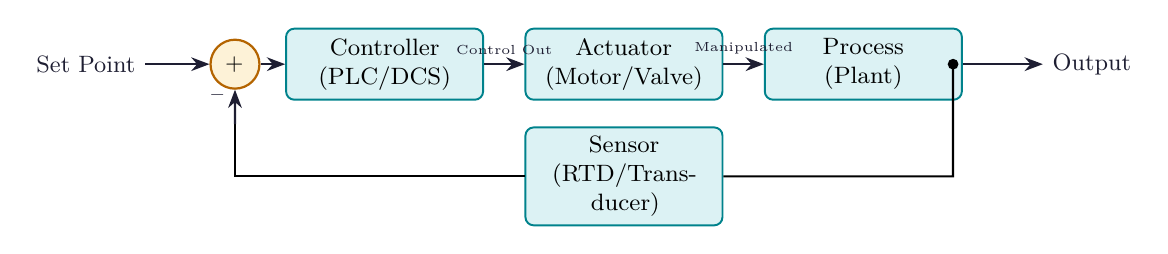
\begin{tikzpicture}[scale=0.95, transform shape]
  \node[block] (ctrl) at (0,0) {Controller\\(PLC/DCS)};
  \node[block] (act) at (3.2,0) {Actuator\\(Motor/Valve)};
  \node[block] (proc) at (6.4,0) {Process\\(Plant)};
  \node[block] (sens) at (3.2,-1.5) {Sensor\\(RTD/Transducer)};
  \node[sumjunc] (sum) at (-2.0,0) {$+$};

  % Paths
  \draw[arrow] (-3.2, 0) node[left, font=\small] {Set Point} -- (sum);
  \draw[arrow] (sum) -- (ctrl);
  \draw[arrow] (ctrl) -- (act) node[midway, above, font=\tiny] {Control Out};
  \draw[arrow] (act) -- (proc) node[midway, above, font=\tiny] {Manipulated};
  \draw[arrow] (proc) -- (8.8, 0) node[right, font=\small] {Output};
  
  \draw[thick] (7.6,0) to[short, *-] (7.6,-1.5) -- (sens);
  \draw[thick] (sens) -| (-2.0,-0.8);
  \draw[arrow] (-2.0,-0.8) -- (sum) node[left, pos=0.8, font=\scriptsize] {$-$};
\end{tikzpicture}
\end{tcolorbox}

% ===============================================================================
\section{Industrial Displacement and Force Sensors}
% ===============================================================================

\subsection{1. Linear Variable Differential Transformer (LVDT)}
An \textbf{LVDT} is an inductive, passive transducer that converts linear displacement into a proportional AC voltage.
\begin{itemize}[leftmargin=*, itemsep=2pt]
  \item \textbf{Structure:} Consists of a single primary winding ($P$) and two identical secondary windings ($S_1$ and $S_2$) wound symmetrically on a hollow cylindrical coil form, with a highly permeable nickel-iron magnetic core sliding inside.
\end{itemize}

\begin{tcolorbox}[tikzbox, title={LVDT Block Structure and Coil Connections}]
\centering
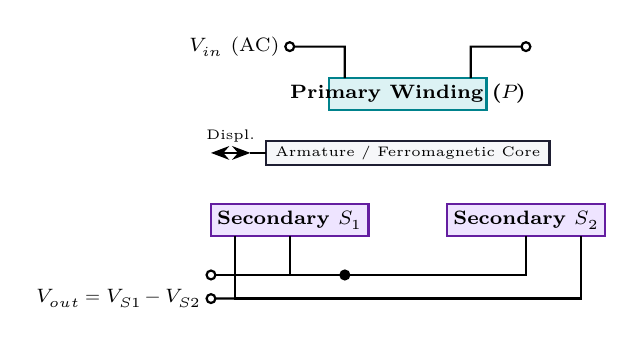
\begin{tikzpicture}[scale=1.0]
  % Primary coil
  \draw[thick, fill=hdrteal, draw=myteal] (-1.0, 0.6) rectangle (1.0, 1.0);
  \node[font=\scriptsize\bfseries] at (0, 0.8) {Primary Winding ($P$)};
  
  % Secondary coil 1
  \draw[thick, fill=hdrpurple, draw=mypurple] (-2.5, -0.6) rectangle (-0.5, -1.0);
  \node[font=\scriptsize\bfseries] at (-1.5, -0.8) {Secondary $S_1$};
  
  % Secondary coil 2
  \draw[thick, fill=hdrpurple, draw=mypurple] (0.5, -0.6) rectangle (2.5, -1.0);
  \node[font=\scriptsize\bfseries] at (1.5, -0.8) {Secondary $S_2$};
  
  % Core shaft
  \draw[thick, fill=mygray, draw=mydark] (-1.8, -0.1) rectangle (1.8, 0.2);
  \node[font=\tiny] at (0, 0.05) {Armature / Ferromagnetic Core};
  
  \draw[thick, Stealth-Stealth] (-2.5, 0.05) -- (-2.0, 0.05) node[midway, above, font=\tiny] {Displ.};
  \draw[thick] (-2.0, 0.05) -- (-1.8, 0.05);

  % Winding electrical connection
  \draw[thick] (-1.5, -1.0) -- (-1.5, -1.5) -- (-0.8, -1.5) to[short, *-] (0.8, -1.5) -- (1.5, -1.5) -- (1.5, -1.0);
  \draw[thick] (-2.2, -1.0) -- (-2.2, -1.8) -- (2.2, -1.8) -- (2.2, -1.0);
  \draw[thick] (-2.2, -1.8) to[short, -o] (-2.5, -1.8) node[left, font=\scriptsize] {$V_{out} = V_{S1} - V_{S2}$};
  \draw[thick] (-1.5, -1.5) to[short, -o] (-2.5, -1.5);
  
  % AC supply to primary
  \draw[thick] (-0.8, 1.0) -- (-0.8, 1.4) to[short, -o] (-1.5, 1.4) node[left, font=\scriptsize] {$V_{in}$ (AC)};
  \draw[thick] (0.8, 1.0) -- (0.8, 1.4) to[short, -o] (1.5, 1.4);
\end{tikzpicture}
\end{tcolorbox}

\textbf{Working Principle:}
\begin{enumerate}[label=\textbf{\alph*.}, leftmargin=*]
  \item An AC excitation voltage $V_{in}(t) = V_p \sin(\omega t)$ is applied to the primary winding. This generates an alternating magnetic field that induces voltages $V_{s1}$ and $V_{s2}$ in the secondaries.
  \item The secondary windings are connected in \textbf{series opposition}, so the net output voltage is:
  \[
  V_{out} = V_{s1} - V_{s2}
  \]
  \item \textbf{Null Position:} When the core is centered, the magnetic coupling to both secondaries is equal, so $V_{s1} = V_{s2}$ and $V_{out} = 0$.
  \item \textbf{Displacement:} When the core moves toward $S_1$, the coupling to $S_1$ increases and $S_2$ decreases ($V_{s1} > V_{s2}$), so $V_{out}$ is in-phase with $V_{in}$. When the core moves toward $S_2$, $V_{s2} > V_{s1}$ and $V_{out}$ is $180^\circ$ out-of-phase with $V_{in}$.
\end{enumerate}

\subsection{2. Potentiometric Sensors \& Loading Effect}
A potentiometer consists of a resistive element with a sliding wiper. The output voltage is proportional to wiper position.
\begin{itemize}[leftmargin=*, itemsep=2pt]
  \item \textbf{Loading Effect:} When a voltmeter or load resistor $R_L$ is connected across the wiper output, it draws current. This causes the output voltage $V_{out}$ to drop below the ideal linear value.
  \item \textbf{Derivation:} Let $R_p$ be the total resistance and $x \in [0, 1]$ be the fractional wiper position. The resistance of the tapped portion is $x R_p$, and the remaining portion is $(1-x)R_p$. The parallel combination of $x R_p$ and $R_L$ is:
  \[
  R_p' = \frac{x R_p R_L}{x R_p + R_L}
  \]
  Applying the voltage divider rule:
  \[
  V_{out} = V_{in} \frac{R_p'}{R_p' + (1-x)R_p} = V_{in} \frac{x}{x + (1-x)(1 + x \frac{R_p}{R_L})} = V_{in} \frac{x}{1 + x(1-x)\frac{R_p}{R_L}}
  \]
  If $R_L \gg R_p$, the denominator approaches 1, yielding the ideal linear relationship $V_{out} \approx x V_{in}$.
\end{itemize}

\subsection{3. Strain Gauges \& Gauge Factor Derivation}
A strain gauge is a resistive sensor whose resistance changes when subjected to mechanical strain.
\begin{tcolorbox}[defbox, title={\textbf{Piezoresistive Effect and Strain}}]
Strain ($\epsilon = \Delta L / L$) causes a change in the physical dimensions (length, area) and the electrical resistivity ($\rho$) of the gauge material, resulting in a fractional change in resistance $\Delta R / R$.
\end{tcolorbox}

\textbf{Derivation of Gauge Factor ($GF$):}
Resistance of a conductor of length $L$, cross-sectional area $A$, and resistivity $\rho$ is:
\[
R = \frac{\rho L}{A}
\]
Taking the natural logarithm on both sides:
\[
\ln R = \ln \rho + \ln L - \ln A
\]
Differentiating both sides:
\[
\frac{dR}{R} = \frac{d\rho}{\rho} + \frac{dL}{L} - \frac{dA}{A}
\]
For a cylindrical wire of diameter $D$, $A = \frac{\pi D^2}{4} \Rightarrow \ln A = \ln\left(\frac{\pi}{4}\right) + 2\ln D$. Differentiating yields:
\[
\frac{dA}{A} = 2 \frac{dD}{D}
\]
Poisson's ratio $\nu$ relates lateral strain to longitudinal strain:
\[
\nu = -\frac{dD/D}{dL/L} \Rightarrow \frac{dD}{D} = -\nu \frac{dL}{L} \Rightarrow \frac{dA}{A} = -2\nu \frac{dL}{L}
\]
Substitute $\frac{dA}{A}$ back into the resistance equation:
\[
\frac{dR}{R} = \frac{dL}{L} - \left(-2\nu \frac{dL}{L}\right) + \frac{d\rho}{\rho} = \frac{dL}{L}(1 + 2\nu) + \frac{d\rho}{\rho}
\]
Dividing by longitudinal strain $\epsilon = dL/L$, we obtain the \textbf{Gauge Factor ($GF$)}:
\begin{tcolorbox}[formulabox, title={\textbf{Gauge Factor Equation}}]
\[
GF = \frac{dR/R}{\epsilon} = 1 + 2\nu + \frac{d\rho/\rho}{\epsilon}
\]
\end{tcolorbox}
Here, $1$ represents change in length, $2\nu$ represents change in area, and $\frac{d\rho/\rho}{\epsilon}$ represents the piezoresistive effect (dominant in semiconductors). For metal gauges, $GF \approx 2$; for semiconductor gauges, $GF \approx 100\text{--}150$.

\subsection{4. Load Cells \& Wheatstone Bridge Readout}
A load cell consists of strain gauges bonded to an elastic metal block. When a force is applied, the block deforms, creating strain. To measure the tiny resistance changes ($\sim 0.1\%$) and reject temperature effects, the strain gauges are wired in a Wheatstone bridge.

\begin{tcolorbox}[tikzbox, title={Wheatstone Bridge Strain Gauge Readout Circuit}]
\centering
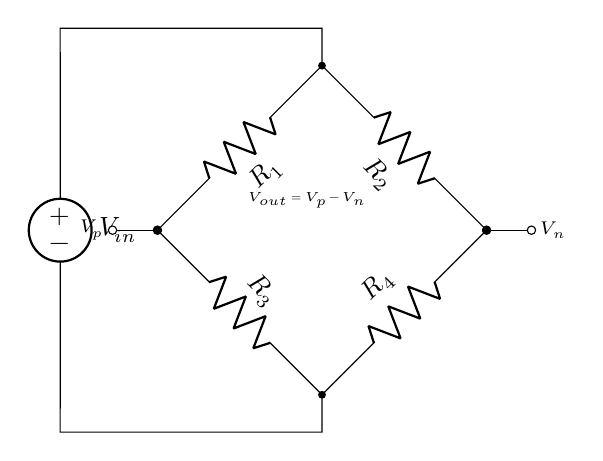
\begin{tikzpicture}[scale=0.95, transform shape]
  % Bridge nodes
  \coordinate (top) at (0, 2.2);
  \coordinate (bottom) at (0, -2.2);
  \coordinate (left) at (-2.2, 0);
  \coordinate (right) at (2.2, 0);

  % Resistors
  \draw (top) to[R, l=$R_1$] (left);
  \draw (left) to[R, l=$R_3$] (bottom);
  \draw (top) to[R, l_=$R_2$] (right);
  \draw (right) to[R, l_=$R_4$] (bottom);

  % Source
  \draw (top) -- (0, 2.7) -- (-3.5, 2.7) to[V, l=$V_{in}$] (-3.5, -2.7) -- (0, -2.7) -- (bottom);
  \fill (top) circle (1.5pt) (bottom) circle (1.5pt);
  
  % Outputs
  \draw (left) to[short, *-o] (-2.8, 0) node[left, font=\scriptsize] {$V_p$};
  \draw (right) to[short, *-o] (2.8, 0) node[right, font=\scriptsize] {$V_n$};
  
  \node[font=\tiny] at (-0.2, 0.4) {$V_{out} = V_p - V_n$};
\end{tikzpicture}
\end{tcolorbox}

For a balanced bridge with $R_1=R_2=R_3=R_4=R$, if active gauges experience strain ($\Delta R$), the output voltage is:
\begin{itemize}[leftmargin=*, itemsep=2.5pt]
  \item \textbf{Quarter Bridge (1 active gauge):} $V_{out} = V_{in} \frac{\Delta R}{4R} = \frac{GF \cdot \epsilon}{4} V_{in}$
  \item \textbf{Half Bridge (2 active gauges):} $V_{out} = V_{in} \frac{\Delta R}{2R} = \frac{GF \cdot \epsilon}{2} V_{in}$
  \item \textbf{Full Bridge (4 active gauges):} $V_{out} = V_{in} \frac{\Delta R}{R} = GF \cdot \epsilon \cdot V_{in}$ (highest sensitivity and full temperature compensation).
\end{itemize}

\subsection{5. Ultrasonic Sensors}
Ultrasonic sensors transmit high-frequency sound bursts ($\sim 40\,$kHz) and measure the echo return time to compute distance based on the \textbf{Time-of-Flight (ToF)} principle:
\begin{tcolorbox}[formulabox, title={\textbf{ToF Distance Equation}}]
\[
d = \frac{v \times t}{2}
\]
\end{tcolorbox}
where $d$ is the distance (m), $t$ is the elapsed time (s), and $v$ is the velocity of sound in the air. 
Sound velocity changes with temperature: $v \approx 331.4 + 0.607 T_C \text{ m/s}$ (where $T_C$ is the temperature in $^\circ$C). Hence, industrial level sensors include an integrated temperature sensor for real-time calibration.


% ===============================================================================
\section{Industrial Temperature and Pressure Sensors}
% ===============================================================================

\subsection{1. Resistance Temperature Detectors (RTD)}
RTDs are temperature sensors containing metallic elements whose resistance increases linearly with temperature (positive temperature coefficient).
\begin{itemize}[leftmargin=*, itemsep=2pt]
  \item \textbf{PT100:} The most common RTD, made of Platinum, having a nominal resistance of $100\,\Omega$ at $0^\circ$C, with a temperature coefficient $\alpha = 0.00385\,\Omega/\Omega/^\circ$C.
  \item \textbf{Linear Model:} For moderate temperature ranges ($0$ to $100^\circ$C):
  \[
  R(T) = R_0 (1 + \alpha T)
  \]
  \item \textbf{Self-Heating:} Since RTDs are resistive, the excitation current $I_{ex}$ creates $I_{ex}^2 R$ power dissipation, heating the element and causing a measurement error. To minimize this, $I_{ex}$ is limited to $< 1\,$mA in industrial transmitter circuits.
\end{itemize}

\subsection{2. Thermistors}
Thermistors are semiconductor-based temperature sensors that exhibit highly non-linear resistance changes.
\begin{itemize}[leftmargin=*, itemsep=2.5pt]
  \item \textbf{NTC (Negative Temperature Coefficient):} Resistance drops exponentially as temperature rises. Extremely sensitive over narrow ranges (e.g., $-50$ to $150^\circ$C).
  \item \textbf{Steinhart-Hart Equation:} The accurate non-linear model:
  \[
  \frac{1}{T} = A + B \ln R + C (\ln R)^3
  \]
  where $T$ is in Kelvin, and $A, B, C$ are curve-fitting constants.
  \item \textbf{PTC (Positive Temperature Coefficient):} Resistance increases sharply at a switching temperature. Used for overcurrent protection.
\end{itemize}

\subsection{3. Thermocouples}
A thermocouple consists of two dissimilar metal wires joined at one end (hot junction). When a temperature difference exists between the hot junction ($T_h$) and the open cold junction ($T_c$), an electromotive force (emf) is generated (Seebeck effect).
\begin{itemize}[leftmargin=*, itemsep=2.5pt]
  \item \textbf{Seebeck Voltage:}
    \[
    V_{out} = \alpha_{S} (T_h - T_c)
    \]
    where $\alpha_{S}$ is the material Seebeck coefficient ($\mu$V/$^\circ$C).
  \item \textbf{Cold Junction Compensation (CJC):} The thermocouple only measures the temperature difference $(T_h - T_c)$. To determine $T_h$, the temperature of the cold junction terminal board $T_c$ must be measured independently (using an RTD or thermistor), and the corresponding Seebeck voltage is added mathematically to the thermocouple signal.
\end{itemize}

\subsection{4. Pressure Sensors}
\begin{itemize}[leftmargin=*, itemsep=2.5pt]
  \item \textbf{Piezoelectric Pressure Sensors:} Quartz crystals generate an electrical charge $q$ when subjected to mechanical force/pressure:
    \[
    q = d \cdot F = d \cdot A \cdot P
    \]
    where $d$ is the piezoelectric charge constant, $F$ is force, $A$ is area, and $P$ is pressure. Suitable for dynamic pressure changes only (charge leaks away under static pressure).
  \item \textbf{Capacitive Pressure Sensors:} A flexible metal diaphragm acts as one plate of a capacitor. Applied pressure deforms the diaphragm, changing the plate spacing $d$, which alters the capacitance:
    \[
    C = \frac{\epsilon_0 \epsilon_r A}{d - \Delta d}
    \]
    Extremely stable and used for static industrial gauge/differential pressure transmitters.
\end{itemize}

% ===============================================================================
\section{Industrial Actuators}
% ===============================================================================

\subsection{1. DC Motors and Speed Control}
DC motors convert electrical energy to rotational torque. Speed control is achieved by varying the average armature voltage using \textbf{Pulse-Width Modulation (PWM)}.

\textbf{H-Bridge Driver:} Consists of 4 electronic switches (MOSFETs) that steer current through the armature. Toggling diagonal switch pairs allows bidirectional rotation and braking.

\subsection{2. Stepper Motors}
A stepper motor divides a full rotation into a series of equal angular increments (steps).
\begin{itemize}[leftmargin=*, itemsep=2.5pt]
  \item \textbf{Step Angle ($\theta_s$):}
    \[
    \theta_s = \frac{360^\circ}{N_s \times N_r} = \frac{360^\circ}{\text{Number of Phases} \times \text{Rotor Teeth}}
    \]
  \item \textbf{Microstepping:} By driving the stator phases with sine-cosine current profiles instead of full steps, the rotor can be positioned at intermediate angles, reducing vibration and achieving sub-degree step resolution.
\end{itemize}

\subsection{3. Servo Motors}
A servo motor is a rotary actuator that couples a standard motor (DC or AC) with a position feedback sensor (encoder) and a closed-loop controller. The controller continuously adjusts the motor drive voltage based on the error between the commanded position and the actual position.

\subsection{4. Piezoelectric Actuators}
Piezoelectric actuators use the \textbf{inverse piezoelectric effect} to produce minute displacements (nanometer scale) when an electric field is applied. Extremely high force capability but very short stroke lengths (typically $<100\,\mu$m). Used in precision micro-positioning and optical alignment.

\subsection{5. Pneumatic Actuators}
Pneumatic systems convert compressed air energy into linear or rotary motion.
\begin{itemize}[leftmargin=*, itemsep=2.5pt]
  \item \textbf{Double-Acting Cylinder:} Air is routed to one chamber to extend the piston, while exhausting air from the other. To retract the piston, the air connections are reversed.
  \item \textbf{Directional Control Valves (DCV):} A 5-port, 2-position (5/2) valve is the industrial standard for controlling double-acting cylinders.
\end{itemize}

\begin{tcolorbox}[tikzbox, title={Pneumatic Control System with a 5/2 Valve and Double-Acting Cylinder}]
\centering
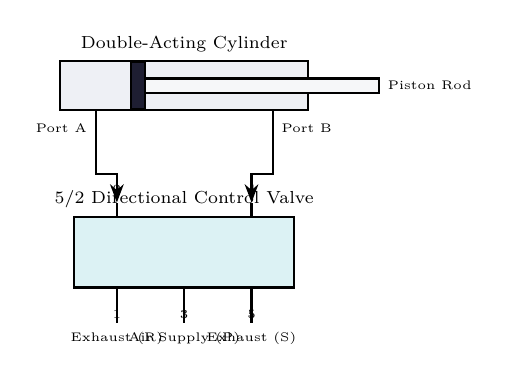
\begin{tikzpicture}[scale=0.9, transform shape]
  % Cylinder body
  \draw[thick, fill=hdrgray] (0, 0.5) rectangle (3.5, 1.2);
  \node[above, font=\scriptsize] at (1.75, 1.2) {Double-Acting Cylinder};
  
  % Piston and rod
  \draw[thick, fill=mydark] (1.0, 0.52) rectangle (1.2, 1.18);
  \draw[thick, fill=mygray] (1.2, 0.75) rectangle (4.5, 0.95);
  \node[right, font=\tiny] at (4.5, 0.85) {Piston Rod};
  
  % Ports
  \draw[thick] (0.5, 0.5) -- (0.5, 0.0);
  \draw[thick] (3.0, 0.5) -- (3.0, 0.0);
  \node[left, font=\tiny] at (0.5, 0.25) {Port A};
  \node[right, font=\tiny] at (3.0, 0.25) {Port B};

  % Valve housing
  \begin{scope}[yshift=-2.0cm]
    \draw[thick, fill=hdrteal] (0.2, 0) rectangle (3.3, 1.0);
    \node[above, font=\scriptsize] at (1.75, 1.0) {5/2 Directional Control Valve};
    
    % Ports on valve
    \draw[thick] (0.8, 1.0) -- (0.8, 1.2); \node[above, font=\tiny] at (0.8, 1.2) {2};
    \draw[thick] (2.7, 1.0) -- (2.7, 1.2); \node[above, font=\tiny] at (2.7, 1.2) {4};
    
    \draw[thick] (0.8, 0) -- (0.8, -0.2); \node[below, font=\tiny] at (0.8, -0.2) {1};
    \draw[thick] (1.75, 0) -- (1.75, -0.2); \node[below, font=\tiny] at (1.75, -0.2) {3};
    \draw[thick] (2.7, 0) -- (2.7, -0.2); \node[below, font=\tiny] at (2.7, -0.2) {5};
  \end{scope}
  
  % Connections
  \draw[thick, -Stealth] (0.5, 0) -- ++(0, -0.4) -| (0.8, -0.8);
  \draw[thick, -Stealth] (3.0, 0) -- ++(0, -0.4) -| (2.7, -0.8);
  \draw[thick] (0.8, -2.2) -- ++(0, -0.3) node[below, font=\tiny] {Exhaust (R)};
  \draw[thick] (2.7, -2.2) -- ++(0, -0.3) node[below, font=\tiny] {Exhaust (S)};
  \draw[thick] (1.75, -2.2) -- ++(0, -0.3) node[below, font=\tiny] {Air Supply (P)};
\end{tikzpicture}
\end{tcolorbox}

\newpage

% ===============================================================================
% QUICK REVISION PAGE
% ===============================================================================
\begin{center}
  {\large\bfseries\color{myred} Quick Revision --- Module 1}\\[3pt]
  {\small\color{mydark} Sensors \& Actuators $|$ PE-EC802B}
\end{center}
\noindent{\color{myred}\rule{\linewidth}{1.2pt}}
\vspace{4pt}

\begin{tcolorbox}[formulabox, title={\textbf{Key Formulas at a Glance}}]
\renewcommand{\arraystretch}{1.35}
\begin{tabularx}{\linewidth}{B{5.2cm} X}
Potentiometer Loading Error & $V_{out} = V_{in} \frac{x}{1 + x(1-x)\frac{R_p}{R_L}}$ \\[4pt]
Gauge Factor & $GF = \frac{\Delta R / R}{\epsilon} = 1 + 2\nu + \frac{\Delta\rho/\rho}{\epsilon}$ \\[4pt]
RTD Resistance & $R(T) = R_0 (1 + \alpha T)$ \\[4pt]
Steinhart-Hart (Thermistor) & $\frac{1}{T} = A + B \ln R + C (\ln R)^3$ \\[4pt]
Ultrasonic Distance & $d = \frac{v \times t}{2}$ where $v \approx 331.4 + 0.6 T_C$ \\[4pt]
Stepper Step Angle & $\theta_s = \frac{360^\circ}{N_s \times N_r}$ \\
\end{tabularx}
\end{tcolorbox}

\begin{tcolorbox}[defbox, title={\textbf{One-Line Definitions}}]
\begin{itemize}[leftmargin=*, itemsep=2pt, topsep=0pt]
  \item \textbf{LVDT:} A transformer-based passive sensor that outputs an AC voltage proportional to the linear displacement of a sliding core.
  \item \textbf{Gauge Factor:} The ratio of fractional change in resistance to the mechanical strain applied to a strain gauge.
  \item \textbf{Poisson's Ratio ($\nu$):} The ratio of lateral transverse strain to longitudinal axial strain.
  \item \textbf{PT100:} A platinum RTD having $100\,\Omega$ resistance at $0^\circ$C and a standard positive temperature coefficient.
  \item \textbf{Seebeck Effect:} The generation of a voltage at the open terminals of two dissimilar metals due to a temperature difference.
  \item \textbf{Microstepping:} Controlling stepper phases with fractional currents to position the rotor between full steps.
\end{itemize}
\end{tcolorbox}

\begin{tcolorbox}[tikzbox, title={\textbf{Sensor \& Actuator Technology Comparisons}}]
\centering
\par\noindent
\renewcommand{\arraystretch}{1.3}
\begin{tabularx}{\linewidth}{|B{2.8cm}|Y|Y|Y|}
\hline
\textbf{Property} & \textbf{RTD} & \textbf{Thermocouple} & \textbf{Thermistor} \\ \hline
\textbf{Linearity} & Highly Linear & Non-linear & Exponentially Non-linear \\ \hline
\textbf{Temp.~Range} & Wide ($-200$ to $850^\circ$C) & Extremely Wide ($-270$ to $1800^\circ$C) & Narrow ($-50$ to $150^\circ$C) \\ \hline
\textbf{Sensitivity} & Moderate & Low ($\mu$V/$^\circ$C) & Very High ($\Omega$/$^\circ$C) \\ \hline
\textbf{CJC Required} & No & Yes & No \\ \hline
\end{tabularx}

\vspace{0.3cm}
\begin{tabularx}{\linewidth}{|B{2.8cm}|Y|Y|}
\hline
\textbf{Property} & \textbf{Stepper Motor} & \textbf{Servo Motor} \\ \hline
\textbf{Control Mode} & Open-loop (no sensor feedback) & Closed-loop (requires encoder) \\ \hline
\textbf{Torque at Speed} & High at low speed; falls at high speed & Constant torque throughout speed range \\ \hline
\textbf{Precision} & Limited by step angle/microstepping & High (limited only by encoder resolution) \\ \hline
\textbf{Cost \& Complexity} & Low cost; simple drive interface & High cost; complex servo tuning \\ \hline
\end{tabularx}
\end{tcolorbox}

\begin{tcolorbox}[exambox, title={\textbf{Frequently Asked / Viva Questions}}]
\begin{enumerate}[leftmargin=*, itemsep=4pt]
  \item \Q{Why are LVDT secondary windings connected in series opposition?}
    This connection ensures that the induced voltages in the two secondaries ($V_{s1}$ and $V_{s2}$) subtract. When the core is centered, the voltages cancel, producing $V_{out}=0$. This establishes a clear zero reference point (null position) to identify direction and magnitude.
  \item \Q{Explain the role of dummy strain gauges in bridge circuits.}
    Dummy strain gauges are exposed to the same temperature as the active gauge but are not subjected to mechanical strain. By placing them in adjacent bridge arms, temperature-induced resistance changes cancel out, preventing thermal drift errors.
  \item \Q{What is the Seebeck effect, and how is it used in thermocouples?}
    It states that when two junctions of dissimilar metals are at different temperatures, an electrical potential difference (voltage) is generated. Thermocouples use this to measure the temperature difference between the hot and cold junctions.
  \item \Q{Why is 4-wire measurement preferred for RTDs in industrial settings?}
    In 2-wire RTDs, the resistance of the lead wires adds to the measurement, causing a positive temperature error. In 4-wire RTDs, two wires supply a constant current while the other two high-impedance wires measure the voltage across the sensor element, completely eliminating lead resistance error.
  \item \Q{Explain the physical reason behind NTC behavior in thermistors.}
    As temperature increases in a semiconductor material, thermal energy excites more valence electrons into the conduction band. This increases the concentration of free charge carriers, leading to a drop in electrical resistance.
  \item \Q{Compare Full-step, Half-step, and Microstepping in stepper motor control.}
    Full-step drives one or two phases fully, moving the rotor by its full step angle. Half-step toggles between one and two phases, cutting step angle in half. Microstepping applies sine-cosine current profiles to stator coils, positioning the rotor smoothly at intermediate microsteps, reducing vibration.
\end{enumerate}
\end{tcolorbox}


% -- Module 2 -----------------------------------------------------------------
\modulestart{2}{Industrial Signal Conditioning}

\section{Industrial Signal Conditioning}
% ===============================================================================

Physical signals from industrial sensors are usually low-voltage ($\mu$V to mV), high-impedance, and contaminated with common-mode noise. \textbf{Signal conditioning} circuits amplify, filter, and isolate these inputs before conversion.

\subsection{1. Three-Op-Amp Instrumentation Amplifier}
An instrumentation amplifier (IA) is a specialized differential amplifier characterized by extremely high input impedance, low DC offset, and outstanding \textbf{Common-Mode Rejection Ratio (CMRR)}.

\begin{tcolorbox}[tikzbox, title={Three-Op-Amp Instrumentation Amplifier Schematic}]
\centering
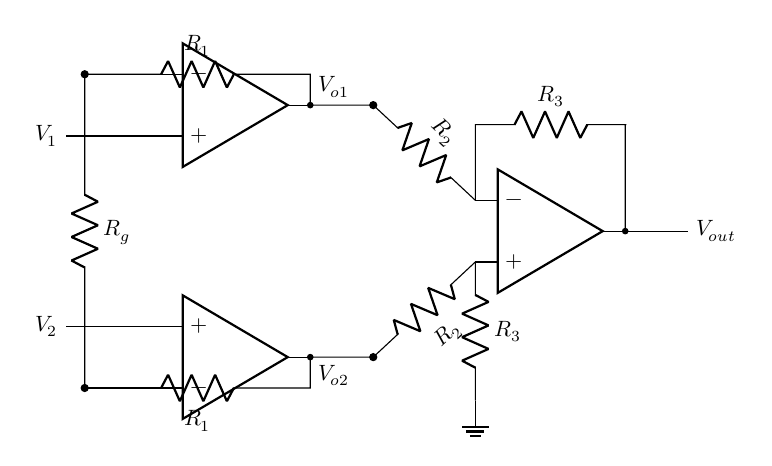
\begin{tikzpicture}[scale=0.8, transform shape]
  % Op-amps
  \draw (0, 2) node[op amp] (op1) {};
  \draw (0, -2) node[op amp, yscale=-1] (op2) {};
  \draw (5, 0) node[op amp] (op3) {};

  % Inputs
  \draw (op1.-) -- ++(-1.2, 0) coordinate (in1_minus);
  \draw (op1.+) -- ++(-1.5, 0) node[left] {$V_1$};
  \draw (op2.-) -- ++(-1.2, 0) coordinate (in2_minus);
  \draw (op2.+) -- ++(-1.5, 0) node[left] {$V_2$};

  % Resistors
  \draw (in1_minus) to[R, l=$R_1$] (op1.out |- op1.-) -- (op1.out);
  \draw (in2_minus) to[R, l_=$R_1$] (op2.out |- op2.-) -- (op2.out);
  \draw (in1_minus) to[R, l=$R_g$, *-*] (in2_minus);

  % Output of first stage nodes
  \fill (op1.out) circle (1.5pt) node[above right] {$V_{o1}$};
  \fill (op2.out) circle (1.5pt) node[below right] {$V_{o2}$};

  % Connections to second stage
  \draw (op1.out) -- ++(1.0, 0) to[R, l=$R_2$, *-] (op3.-);
  \draw (op2.out) -- ++(1.0, 0) to[R, l_=$R_2$, *-] (op3.+);

  % Feedback and reference for second stage
  \draw (op3.-) -- ++(0, 1.2) to[R, l=$R_3$] ++(2.4, 0) -| (op3.out);
  \draw (op3.+) to[R, l=$R_3$] ++(0, -2.2) node[ground] {};

  % Output
  \draw (op3.out) -- ++(1.0, 0) node[right] {$V_{out}$};
  \fill (op3.out) circle (1.5pt);
\end{tikzpicture}
\tcbset{breakable}
\end{tcolorbox}

\textbf{Mathematical Gain Derivation:}
\begin{enumerate}[label=\textbf{\arabic*.}, leftmargin=*]
  \item \textbf{First Stage (Input Buffers):} By virtual ground concept, the voltages at the inverting terminals of $A_1$ and $A_2$ are held at $V_1$ and $V_2$ respectively. Thus, the voltage drop across the gain resistor $R_g$ is:
  \[
  V_{Rg} = V_1 - V_2
  \]
  \item The current flowing through $R_g$ is $I_g = \frac{V_1 - V_2}{R_g}$. Since no current flows into the op-amp terminals, this same current $I_g$ must flow through both feedback resistors $R_1$. The voltage difference between the first-stage outputs $V_{o1}$ and $V_{o2}$ is:
  \[
  V_{o1} - V_{o2} = I_g (R_1 + R_g + R_1) = I_g (2R_1 + R_g)
  \]
  Substitute $I_g$:
  \[
  V_{o1} - V_{o2} = \left(\frac{V_1 - V_2}{R_g}\right) (2R_1 + R_g) = \left(1 + \frac{2R_1}{R_g}\right)(V_1 - V_2)
  \]
  \item \textbf{Second Stage (Differential Amplifier):} The second stage is a standard differential amplifier. Under matched resistor conditions ($R_2$ and $R_3$):
  \[
  V_{out} = \frac{R_3}{R_2}(V_{o2} - V_{o1})
  \]
  \item \textbf{Net Closed-Loop Output Voltage:} Combining the two stage equations yields:
  \begin{tcolorbox}[formulabox, title={\textbf{Instrumentation Amplifier Output Gain}}]
  \[
  V_{out} = \left(1 + \frac{2R_1}{R_g}\right)\left(\frac{R_3}{R_2}\right)(V_2 - V_1)
  \]
  \end{tcolorbox}
  By adjusting only a single external resistor $R_g$, the differential gain can be tuned across a wide range without upsetting resistor matching or input impedance.
\end{enumerate}

\subsection{2. Sallen-Key Active Filtering}
Active filters reject high-frequency noise while buffering signals. The Sallen-Key topology is the standard second-order active filter.

\textbf{Transfer Function (2nd-Order Low-Pass):}
\[
H(s) = \frac{V_{out}(s)}{V_{in}(s)} = \frac{K}{s^2(R_1 R_2 C_1 C_2) + s(R_1 C_2 + R_2 C_2 + R_1 C_1(1-K)) + 1}
\]
where $K$ is the passband gain. Sallen-Key is highly preferred due to its low component count and minimal sensitivity to op-amp bandwidth limitations.

\subsection{3. Electrical Isolation \& Protection}
Ground loops and common-mode voltage surges can damage control equipment. Isolation breaks physical copper connections while passing the signal.
\begin{itemize}[leftmargin=*, itemsep=2.5pt]
  \item \textbf{Optocouplers (Optical Isolation):} A transmitter LED converts the electrical input into light, which crosses a dielectric barrier to turn on a phototransistor on the receiver side. Provides up to $5\,$kV isolation.
  \item \textbf{Sensor Protection Circuits:} TVS (Transient Voltage Suppressor) diodes and clamping diodes shunt transient voltage spikes (such as electrostatic discharge or inductive switching surges) to power rails/ground, protecting sensitive ADC inputs.
\end{itemize}

\subsection{4. Analog-to-Digital and Digital-to-Analog Converters (ADC \& DAC)}
In computer-based automation (like PLCs or DCS), analog field signals must be digitized by an \textbf{Analog-to-Digital Converter (ADC)} for processor execution, and control outputs must be converted back to analog by a \textbf{Digital-to-Analog Converter (DAC)} to drive actuators.

\textbf{1. ADC Resolution and Quantization:}
An $N$-bit ADC maps a continuous voltage range $V_{FSR}$ to $2^N$ discrete digital states.
\begin{itemize}[leftmargin=*, itemsep=2pt]
  \item \textbf{LSB Size (Resolution):} Represents the smallest voltage change that can be resolved:
  \begin{tcolorbox}[formulabox, title={\textbf{ADC LSB Resolution}}]
  \[
  LSB = \frac{V_{FSR}}{2^N}
  \]
  \end{tcolorbox}
  \item \textbf{Quantization Error:} The error introduced by rounding a continuous voltage to the nearest discrete level. For an ideal ADC, the quantization error $e_q$ is bounded by:
  \[
  e_q \le \pm \frac{1}{2} LSB = \pm \frac{V_{FSR}}{2^{N+1}}
  \]
\end{itemize}

\textbf{2. Industrial ADC Architectures:}
\begin{itemize}[leftmargin=*, itemsep=2.5pt]
  \item \textbf{Successive Approximation Register (SAR) ADC:}
    \begin{itemize}[leftmargin=*, itemsep=1.5pt]
      \item \textit{Working:} Uses a binary search algorithm and an internal DAC to compare the input voltage against successive fractions of the reference voltage. It takes $N$ clock cycles for $N$-bit conversion.
      \item \textit{Characteristics:} Moderate speed (kSPS to MSPS), good resolution (8--18 bits), zero latency. Standard in PLC analog input modules.
    \end{itemize}
  \item \textbf{Sigma-Delta ($\Sigma\Delta$) ADC:}
    \begin{itemize}[leftmargin=*, itemsep=1.5pt]
      \item \textit{Working:} Employs oversampling, 1-bit delta-modulation, noise shaping (pushing quantization noise to high frequencies), and digital decimation filtering to retrieve ultra-precise digital representations.
      \item \textit{Characteristics:} Extremely high resolution (16--24 bits), high noise immunity, slow conversion speed. Ideal for precision weighing systems (load cells) and temperature transmitters (RTDs/Thermocouples).
    \end{itemize}
\end{itemize}

\textbf{3. Industrial DAC Architectures:}
\begin{itemize}[leftmargin=*, itemsep=2.5pt]
  \item \textbf{Binary-Weighted Resistor DAC:} Uses resistors scaled in binary powers ($R, 2R, 4R, \dots, 2^N R$). The sum of currents at the summing junction is proportional to the binary input.
    \begin{itemize}[leftmargin=*, itemsep=1.5pt]
      \item \textit{Limitation:} For high resolutions, the required ratio of resistor values becomes extremely large (e.g., $1:1024$ for 10-bit), making it practically impossible to fabricate on silicon with matched temperature coefficients.
    \end{itemize}
  \item \textbf{R-2R Ladder DAC:} Uses only two values of precision resistors ($R$ and $2R$).
    \begin{itemize}[leftmargin=*, itemsep=1.5pt]
      \item \textit{Advantage:} Highly scalable, easy to match and fabricate on silicon. It is the dominant architecture used in industrial control DAC modules.
    \end{itemize}
\end{itemize}

\textbf{4. DAC Parameters:}
\begin{itemize}[leftmargin=*, itemsep=2.5pt]
  \item \textbf{Differential Non-Linearity (DNL):} The difference between the actual step size and the ideal 1 LSB step size. A DNL $< -1\,$LSB can cause \textbf{non-monotonicity} (meaning the analog output decreases when the digital input increases).
  \item \textbf{Integral Non-Linearity (INL):} The maximum deviation of the actual transfer function from a straight line connecting the end points. Represents the overall linearity limit.
  \item \textbf{Settling Time:} The time required for the DAC output to settle within $\pm 0.5\,$LSB of its final value following a full-scale digital input transition. Limits output update rate.
\end{itemize}

% ===============================================================================
\section{Industrial Data Transmission and Noise Suppression}
% ===============================================================================

\subsection{1. 4--20 mA Current Loops}
In industrial plants, transmitting analog signals over long distances as voltages causes errors due to the resistance of the lead wires ($I R$ drop) and noise pickup. The \textbf{4--20 mA current loop} standard represents variables as current levels, making the loop immune to line resistance.

\begin{tcolorbox}[tikzbox, title={4--20 mA Industrial Current Loop Model}]
\centering
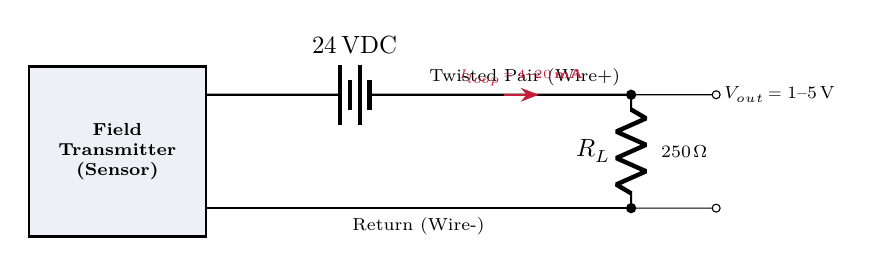
\begin{tikzpicture}[scale=0.9, transform shape]
  % Transmitter Block
  \draw[thick, fill=hdrgray] (-3.5, 1.2) rectangle (-1.0, -1.2);
  \node[font=\scriptsize\bfseries, align=center] at (-2.25, 0) {Field\\Transmitter\\(Sensor)};

  % Cable loop with loop power supply in series
  \draw[thick] (-1.0, 0.8) -- (0.4, 0.8) to[battery, l=$24\,$VDC] (1.8, 0.8) -- (5.0, 0.8);
  \node[above, font=\scriptsize] at (3.5, 0.8) {Twisted Pair (Wire+)};
  \draw[thick] (-1.0, -0.8) -- (5.0, -0.8) node[midway, below, font=\scriptsize] {Return (Wire-)};
  
  % Receiver Resistor
  \draw[thick] (5.0, 0.8) to[R, l_=$R_L$, *-*] (5.0, -0.8);
  \node[right, font=\scriptsize] at (5.3, 0) {$250\,\Omega$};
  \draw (5.0, 0.8) to[short, -o] (6.2, 0.8) node[right, font=\scriptsize] {$V_{out} = 1\text{--}5\,$V};
  \draw (5.0, -0.8) to[short, -o] (6.2, -0.8);
  
  % Loop current arrow
  \draw[-Stealth, thick, color=myred] (3.2, 0.8) -- (3.7, 0.8) node[above, midway, font=\tiny\bfseries] {$I_{loop} = 4\text{--}20\,$mA};
\end{tikzpicture}
\end{tcolorbox}

\textbf{Key Characteristics:}
\begin{enumerate}[label=\textbf{\alph*.}, leftmargin=*]
  \item \textbf{Zero Reference (4 mA):} A loop current of $4\,$mA represents the minimum scale (0\%). This "live zero" allows the controller to distinguish a true zero reading from a broken wire or loop power failure (0 mA).
  \item \textbf{Full Scale (20 mA):} Represents the maximum scale (100%).
  \item \textbf{Receiver Conversion:} At the controller side, the loop current passes through a precision $250\,\Omega$ load resistor $R_L$ to convert the current back into a voltage for the ADC:
  \[
  V_{out} = I_{loop} \times R_L
  \]
  \begin{itemize}[leftmargin=*, itemsep=2pt]
    \item For $I_{loop} = 4\,\text{mA} \Rightarrow V_{out} = 4\,\text{mA} \times 250\,\Omega = 1\,\text{V}$.
    \item For $I_{loop} = 20\,\text{mA} \Rightarrow V_{out} = 20\,\text{mA} \times 250\,\Omega = 5\,\text{V}$.
  \end{itemize}
  The resulting voltage range is a standard $1\text{--}5\,$V.
\end{enumerate}

\subsection{2. RS-485 Differential Data Transmission}
For digital communication in noisy industrial environments (e.g., Modbus protocol), RS-485 is the standard.
\begin{itemize}[leftmargin=*, itemsep=2.5pt]
  \item \textbf{Differential Signaling:} Routes data on two complementary lines ($A$ and $B$). The receiver detects only the difference $V_A - V_B$. Common-mode noise coupled onto the cable affects both lines equally and is rejected.
  \item \textbf{Termination Resistors:} A $120\,\Omega$ resistor is placed at both physical ends of the twisted pair network to match the cable's characteristic impedance, preventing signal reflections that corrupt data.
\end{itemize}

\subsection{3. Grounding and Shielding}
\begin{itemize}[leftmargin=*, itemsep=2.5pt]
  \item \textbf{Ground Loops:} When multiple devices are grounded at different physical locations, differences in ground potential drive a stray current through the ground loop wire, creating noise. Mitigated by using a single-point star ground or isolating signal paths.
  \item \textbf{Electrostatic Shielding:} Enclosing signal conductors in a conductive copper braid or foil shield connected to ground to shunt capacitive noise currents. The shield must be grounded at \textbf{one end only} to avoid creating a ground loop.
\end{itemize}

% ===============================================================================
\section{Errors, Calibration, and Uncertainty}
% ===============================================================================

\subsection{1. Error Categorization}
\begin{itemize}[leftmargin=*, itemsep=2.5pt]
  \item \textbf{Systematic (Deterministic) Errors:} Consistently bias measurements in one direction (e.g., calibration drift, scale offset, loading errors). Can be compensated for via calibration.
  \item \textbf{Random (Stochastic) Errors:} Caused by unpredictable, statistical fluctuations (e.g., thermal noise, electromagnetic interference). Analyzed using probability and mitigated by averaging.
\end{itemize}

\subsection{2. Calibration (Zero and Span Adjustments)}
Calibration is the process of adjusting a sensor's output to match known reference inputs.
\begin{itemize}[leftmargin=*, itemsep=2.5pt]
  \item \textbf{Zero Adjustment:} Shifts the entire calibration curve vertically to set the output to the correct zero value (e.g., setting output to 4 mA when input pressure is 0 psi).
  \item \textbf{Span (Gain) Adjustment:} Tilts the calibration curve by adjusting its slope to set the correct full-scale value (e.g., setting output to 20 mA when input pressure is at maximum).
\end{itemize}

\subsection{3. Uncertainty Propagation}
When a quantity $Y$ is calculated from independent measured values $X_1, X_2, \dots, X_N$ using a function $Y = f(X_1, X_2, \dots, X_N)$, the absolute uncertainty $u_Y$ is:
\begin{tcolorbox}[formulabox, title={\textbf{Uncertainty Propagation Equation}}]
\[
u_Y = \sqrt{\sum_{i=1}^N \left(\frac{\partial f}{\partial X_i} u_{X_i}\right)^2}
\]
\end{tcolorbox}
where $u_{X_i}$ is the standard uncertainty of variable $X_i$.

\newpage

% ===============================================================================
% QUICK REVISION PAGE
% ===============================================================================
\begin{center}
  {\large\bfseries\color{myred} Quick Revision --- Module 2}\\[3pt]
  {\small\color{mydark} Signal Conditioning $|$ PE-EC802B}
\end{center}
\noindent{\color{myred}\rule{\linewidth}{1.2pt}}
\vspace{4pt}

\begin{tcolorbox}[formulabox, title={\textbf{Key Formulas at a Glance}}]
\renewcommand{\arraystretch}{1.35}
\begin{tabularx}{\linewidth}{B{5.2cm} X}
Instrumentation Amp Gain & $V_{out} = \left(1 + \frac{2R_1}{R_g}\right)\left(\frac{R_3}{R_2}\right)(V_2 - V_1)$ \\[4pt]
Sallen-Key LPF Cut-off Freq & $f_c = \frac{1}{2\pi \sqrt{R_1 R_2 C_1 C_2}}$ \\[4pt]
4--20 mA Loop Volt Conversion & $V_{out} = I_{loop} \times R_L \quad (\text{For PT100/Transmitters})$ \\[4pt]
Uncertainty Propagation & $u_Y = \sqrt{\sum \left(\frac{\partial f}{\partial X_i} u_{X_i}\right)^2}$ \\[4pt]
RS-485 Term. Resistance & $R_T = Z_0 \approx 120\,\Omega$ \\[4pt]
ADC LSB Resolution & $LSB = V_{FSR} / 2^N$ \\[4pt]
ADC Quantization Error & $e_q \le \pm \frac{1}{2} LSB = \pm \frac{V_{FSR}}{2^{N+1}}$ \\
\end{tabularx}
\end{tcolorbox}

\begin{tcolorbox}[defbox, title={\textbf{One-Line Definitions}}]
\begin{itemize}[leftmargin=*, itemsep=2pt, topsep=0pt]
  \item \textbf{Instrumentation Amplifier:} A high-gain differential amplifier with extremely high input impedance and CMRR.
  \item \textbf{Live Zero:} Representing the minimum measurement value by a non-zero current (4 mA) to detect wire breaks.
  \item \textbf{Ground Loop:} An undesirable current loop formed when two points in a circuit are grounded at different potentials.
  \item \textbf{Optocoupler:} A device that uses a light path to transmit signals across an electrical isolation barrier.
  \item \textbf{Span Adjustment:} Calibration step that alters the gain (slope) of the measurement system.
  \item \textbf{Zero Adjustment:} Calibration step that adds a constant bias (offset) to shift the calibration curve.
  \item \textbf{Quantization Error:} The round-off error introduced when a continuous analog voltage is mapped to a discrete digital code.
  \item \textbf{Monotonicity:} A DAC property where the analog output always increases (or remains constant) as the digital input code increases.
\end{itemize}
\end{tcolorbox}

\begin{tcolorbox}[tikzbox, title={\textbf{Industrial Transmission \& Grounding Comparisons}}]
\centering
\par\noindent
\renewcommand{\arraystretch}{1.3}
\begin{tabularx}{\linewidth}{|B{3.0cm}|Y|Y|}
\hline
\textbf{Property} & \textbf{4--20 mA Current Loop} & \textbf{0--10 V Voltage Signaling} \\ \hline
\textbf{Noise Immunity} & Extremely High (immune to line $IR$ drop) & Low (susceptible to electromagnetic noise) \\ \hline
\textbf{Distance Limit} & Up to $3\,$km (limited by loop supply voltage) & Short distances ($<10\,$m, due to line drops) \\ \hline
\textbf{Line Break Detect} & Yes (current falls to 0 mA) & No (cannot distinguish open wire from 0 V) \\ \hline
\textbf{Wiring Cost} & Low (simple twisted pair) & High (requires shielded cables) \\ \hline
\end{tabularx}

\vspace{0.3cm}
\begin{tabularx}{\linewidth}{|B{3.0cm}|Y|Y|}
\hline
\textbf{Property} & \textbf{Single-Point Grounding} & \textbf{Multi-Point Grounding} \\ \hline
\textbf{Configuration} & All grounds connect to a single star point & Devices ground locally to the nearest chassis/earth \\ \hline
\textbf{Ground Loop Risk} & None (no duplicate return paths) & High (ground potential differences drive loops) \\ \hline
\textbf{Best Frequency} & Low frequency ($< 1\,$MHz) & High frequency ($> 10\,$MHz) \\ \hline
\end{tabularx}
\end{tcolorbox}

\begin{tcolorbox}[exambox, title={\textbf{Frequently Asked / Viva Questions}}]
\begin{enumerate}[leftmargin=*, itemsep=4pt]
  \item \Q{Why does the first stage of an instrumentation amplifier have a common-mode gain of unity?}
    In the first stage, the two buffers $A_1$ and $A_2$ are connected via $R_g$. If a common-mode voltage $V_{cm}$ is applied to both inputs ($V_1 = V_2 = V_{cm}$), the voltage across $R_g$ is zero. Hence, no current flows through $R_g$ or $R_1$. The output voltages are $V_{o1} = V_{o2} = V_{cm}$. The differential output is zero, and the common-mode gain is exactly 1.
  \item \Q{Why is 4-20 mA current loop transmission preferred over voltage transmission?}
    Current loop signals are immune to voltage drops caused by long wire resistance ($IR$ drops) and contact resistances. Furthermore, the loop current is unaffected by electromagnetic noise induced in the cabling, making it highly robust in industrial plants.
  \item \Q{Explain the "live zero" concept in 4-20 mA current loops.}
    By setting the zero-point measurement to 4 mA (instead of 0 mA), any physical wire break or power failure causes the current to drop to 0 mA. The PLC controller detects this 0 mA state as a "Loop Fail" alarm rather than a valid zero-scale reading.
  \item \Q{What is the purpose of RS-485 termination resistors, and where are they placed?}
    Termination resistors ($120\,\Omega$) match the cable's characteristic impedance. They are placed at the two extreme physical ends of the RS-485 communication line to prevent electrical signal reflections, which cause data corruption at high speeds.
  \item \Q{Why must a cable shield be grounded at only one end?}
    If a shield is grounded at both ends, any potential difference between the two grounds will drive a current through the shield conductor. This current induces noise in the internal signal wires via magnetic coupling, defeating the purpose of the shield. Grounding it at one end prevents ground loops while maintaining electrostatic shielding.
  \item \Q{State the difference between zero error and span error.}
    A zero error is a constant offset that shifts the entire calibration curve vertically, causing the same error magnitude across the full measurement range. A span error is a gain error that alters the slope of the curve, resulting in an error that increases proportionally with the input value.
  \item \Q{Compare SAR and Sigma-Delta ADCs in terms of speed, resolution, and typical industrial application.}
    SAR (Successive Approximation Register) ADCs offer moderate-to-high speed (up to a few MSPS) and moderate-to-high resolution (8--18 bits) with zero latency, making them ideal for general PLC analog inputs. Sigma-Delta ($\Sigma\Delta$) ADCs offer extremely high resolution (16--24 bits) through oversampling and noise shaping but are much slower, making them ideal for precision sensors like load cells and temperature transmitters.
  \item \Q{Explain the difference between DNL and INL in DACs.}
    DNL (Differential Non-Linearity) measures the deviation of an individual step size from the ideal 1 LSB value; a DNL $< -1\,$LSB can cause non-monotonicity. INL (Integral Non-Linearity) measures the maximum deviation of the actual transfer function from the ideal straight line, representing the overall linearity error of the DAC.
\end{enumerate}
\end{tcolorbox}


% -- Module 3 -----------------------------------------------------------------
\modulestart{3}{PID Control Fundamentals}

\section{PID Control Fundamentals}
% ===============================================================================

A \textbf{PID controller} continuously calculates an error value $e(t) = r(t) - y(t)$ (difference between setpoint and process variable) and applies a correction based on Proportional, Integral, and Derivative terms.

\textbf{Ideal PID Equation (Parallel Form):}
\begin{tcolorbox}[formulabox, title={\textbf{Time-Domain PID Control Equation}}]
\[
u(t) = K_p \left( e(t) + \frac{1}{T_i} \int_{0}^{t} e(\tau) d\tau + T_d \frac{de(t)}{dt} \right)
\]
\end{tcolorbox}
where $K_p$ is proportional gain, $T_i$ is integral time, and $T_d$ is derivative time.

\subsection{1. Physical Action of Control Terms}
\begin{itemize}[leftmargin=*, itemsep=2.5pt]
  \item \textbf{Proportional Action ($K_p e(t)$):} Produces an output proportional to the current error. High $K_p$ speeds up response but leads to oscillation and \textbf{never} eliminates steady-state error (offset).
  \item \textbf{Integral Action ($\frac{K_p}{T_i} \int e\,dt$):} Accumulates past errors over time. It continues to drive the output until the error is reduced to zero, thus eliminating steady-state offset.
  \item \textbf{Derivative Action ($K_p T_d \frac{de}{dt}$):} Predicts future error by measuring the rate of change of error. It provides a damping effect, reducing overshoot and settling time, but amplifies high-frequency noise.
\end{itemize}

\subsection{2. PID Practical Non-Idealities \& Mitigations}
\begin{itemize}[leftmargin=*, itemsep=2.5pt]
  \item \textbf{Integral Windup:} When a large setpoint change occurs, the integrator accumulates error, driving the controller output to saturate. The integrator continues to grow (wind up). When the process variable crosses the setpoint, the actuator remains saturated until the integrator unwinds, causing massive overshoot.
  
  \textit{Mitigation:} \textbf{Anti-windup clamping} disables integration when the controller output saturates.
  \item \textbf{Derivative Kick:} A step change in setpoint $r(t)$ creates an infinite derivative $de/dt$, causing a massive output spike (kick) that stresses actuators.
  
  \textit{Mitigation:} Compute derivative action on the process variable rather than the error: $u_D(t) = -K_p T_d \frac{dy(t)}{dt}$ (\textbf{derivative-on-measurement}).
\end{itemize}

% ===============================================================================
\section{Controller Tuning Methods}
% ===============================================================================

\subsection{1. Ziegler-Nichols (ZN) First Method (Open-Loop)}
Applicable to stable processes that exhibit an S-shaped step response (process reaction curve) characterized by a transport delay (dead time) $L$ and a time constant $T$.

\begin{tcolorbox}[tikzbox, title={Ziegler-Nichols 1st Method Tangent Construction}]
\centering
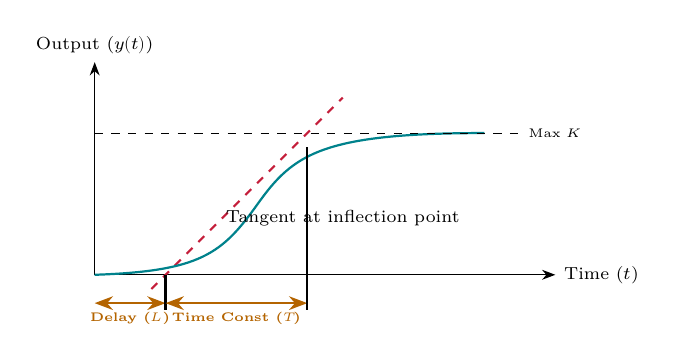
\begin{tikzpicture}[scale=0.9, transform shape]
  % Axes
  \draw[-Stealth, thin] (0,0) -- (6.5,0) node[right, font=\scriptsize] {Time ($t$)};
  \draw[-Stealth, thin] (0,0) -- (0,3.0) node[above, font=\scriptsize] {Output ($y(t)$)};
  
  % Tangent line
  \draw[dashed, color=myred, thick] (0.8, -0.2) -- (3.5, 2.5);
  
  % S-curve
  \draw[thick, color=myteal] (0,0) .. controls (1.5,0.05) and (1.8,0.3) .. (2.3,1.0) .. controls (2.8,1.7) and (3.2,2.0) .. (5.5,2.0);
  \draw[dashed] (0,2.0) -- (6.0,2.0) node[right, font=\tiny] {Max $K$};
  
  % Mark L and T
  \draw[Stealth-Stealth, thick, color=myamber] (0, -0.4) -- (1.0, -0.4) node[midway, below, font=\tiny\bfseries] {Delay ($L$)};
  \draw[thick] (1.0, 0) -- (1.0, -0.5);
  
  \draw[Stealth-Stealth, thick, color=myamber] (1.0, -0.4) -- (3.0, -0.4) node[midway, below, font=\tiny\bfseries] {Time Const ($T$)};
  \draw[thick] (3.0, 1.8) -- (3.0, -0.5);
  
  \node[font=\scriptsize] at (3.5, 0.8) {Tangent at inflection point};
\end{tikzpicture}
\end{tcolorbox}

Let $K$ be the process static gain. The transfer function model is $G(s) = \frac{K e^{-Ls}}{1 + sT}$.
\textbf{Tuning Parameters:}
  \begin{center}
  \small
  \begin{tabularx}{0.85\linewidth}{|B{3.0cm}|Y|Y|Y|}
  \hline
  \textbf{Controller Type} & $K_p$ & $T_i$ & $T_d$ \\ \hline
  \textbf{P} & $T / (KL)$ & $\infty$ & $0$ \\ \hline
  \textbf{PI} & $0.9\,T / (KL)$ & $3.3\,L$ & $0$ \\ \hline
  \textbf{PID} & $1.2\,T / (KL)$ & $2.0\,L$ & $0.5\,L$ \\ \hline
  \end{tabularx}
  \end{center}

\subsection{2. Ziegler-Nichols (ZN) Second Method (Closed-Loop)}
A closed-loop tuning method that increases proportional gain until the loop enters sustained, constant-amplitude oscillations.
\begin{enumerate}[label=\textbf{\arabic*.}, leftmargin=*]
  \item Turn off integral and derivative actions ($T_i = \infty, T_d = 0$).
  \item Increase $K_p$ slowly until the process output oscillates continuously. The gain at this point is the \textbf{Ultimate Gain ($K_u$)}, and the oscillation period is the \textbf{Ultimate Period ($P_u$)}.
\end{enumerate}

\textbf{Tuning Parameters:}
  \begin{center}
  \small
  \begin{tabularx}{0.85\linewidth}{|B{3.0cm}|Y|Y|Y|}
  \hline
  \textbf{Controller Type} & $K_p$ & $T_i$ & $T_d$ \\ \hline
  \textbf{P} & $0.5\,K_u$ & $\infty$ & $0$ \\ \hline
  \textbf{PI} & $0.45\,K_u$ & $0.83\,P_u$ & $0$ \\ \hline
  \textbf{PID} & $0.6\,K_u$ & $0.5\,P_u$ & $0.125\,P_u$ \\ \hline
  \end{tabularx}
  \end{center}

\subsection{3. Cohen-Coon Tuning Method}
Cohen-Coon tuning is designed for systems with a first-order plus dead time (FOPDT) response. Unlike ZN, it provides tuning rules that compensate for processes with large dead times (high ratio of delay $L$ to time constant $T$).
Let $K$ be the static gain, $\tau$ the time constant, and $\theta$ the dead time.
\textbf{Tuning Equations:}
  \begin{itemize}[leftmargin=*, itemsep=3.5pt]
    \item \textbf{PI Controller:}
      \[
      K_p = \frac{\tau}{K\theta} \left( 0.9 + \frac{\theta}{12\tau} \right), \qquad T_i = \theta \frac{30 + 3\theta/\tau}{9 + 20\theta/\tau}
      \]
    \item \textbf{PID Controller:}
      \[
      K_p = \frac{\tau}{K\theta} \left( 1.35 + \frac{\theta}{6\tau} \right), \quad T_i = \theta \frac{32 + 6\theta/\tau}{13 + 8\theta/\tau}, \quad T_d = \theta \frac{4}{11 + 2\theta/\tau}
      \]
  \end{itemize}

% ===============================================================================
\section{Implementation of PID Controllers}
% ===============================================================================

\subsection{1. Analog PID Implementation (Op-Amps)}
Analog controllers use operational amplifiers with capacitors and resistors in parallel branches to implement summing, integrating, and differentiating operations.

\begin{tcolorbox}[tikzbox, title={Analog Op-Amp Parallel PID Controller Circuit}]
\centering
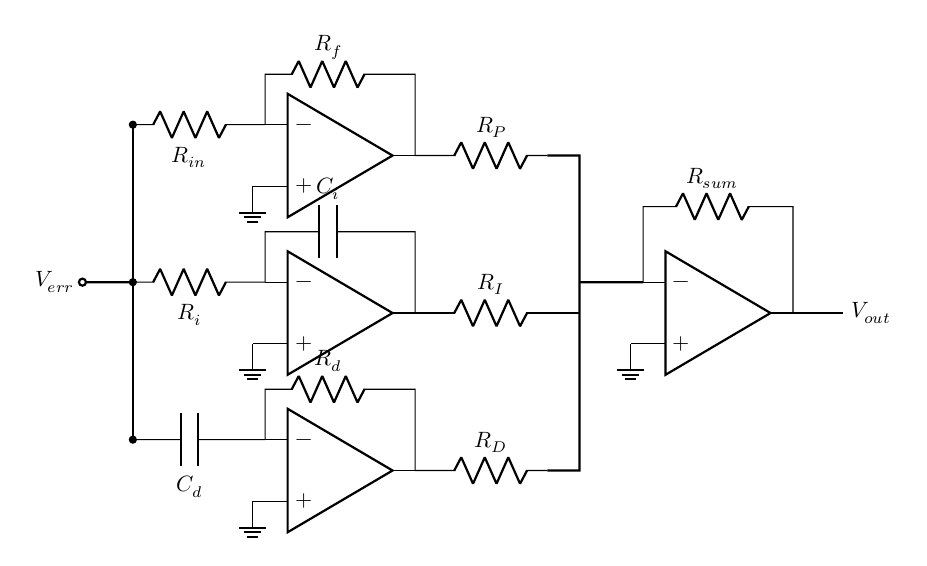
\begin{tikzpicture}[scale=0.8, transform shape]
  % Op-amps aligned at x=0
  \node[op amp] (op1) at (0, 2.5) {};
  \node[op amp] (op2) at (0, 0) {};
  \node[op amp] (op3) at (0, -2.5) {};
  
  % Summing Op-amp (A4)
  \node[op amp] (op4) at (6, 0) {};

  % Proportional Path (A1)
  \draw (op1.+) -- ++(-0.2, 0) node[ground] {};
  \draw (op1.-) -- ++(-0.3, 0) to[R, l=$R_{in}$, -*] ++(-1.8, 0) coordinate (p_in);
  \draw (op1.-) -- ++(0, 0.8) to[R, l=$R_f$] ++(2.0, 0) -| (op1.out);
  \draw (op1.out) -- ++(0.3, 0) to[R, l=$R_P$] ++(1.8, 0) coordinate (p_out);

  % Integral Path (A2)
  \draw (op2.+) -- ++(-0.2, 0) node[ground] {};
  \draw (op2.-) -- ++(-0.3, 0) to[R, l=$R_i$, -*] ++(-1.8, 0) coordinate (i_in);
  \draw (op2.-) -- ++(0, 0.8) to[C, l=$C_i$] ++(2.0, 0) -| (op2.out);
  \draw (op2.out) -- ++(0.3, 0) to[R, l=$R_I$] ++(1.8, 0) coordinate (i_out);

  % Derivative Path (A3)
  \draw (op3.+) -- ++(-0.2, 0) node[ground] {};
  \draw (op3.-) -- ++(-0.3, 0) to[C, l=$C_d$, -*] ++(-1.8, 0) coordinate (d_in);
  \draw (op3.-) -- ++(0, 0.8) to[R, l=$R_d$] ++(2.0, 0) -| (op3.out);
  \draw (op3.out) -- ++(0.3, 0) to[R, l=$R_D$] ++(1.8, 0) coordinate (d_out);

  % Bus lines on input side
  \draw[thick] (p_in) -- (d_in);
  \draw[thick] (i_in) to[short, -o] ++(-0.8, 0) node[left] {$V_{err}$};

  % Summing bus on output side
  \draw[thick] (p_out) -- (3.8, 2.5) -- (3.8, -2.5) -- (d_out);
  \draw[thick] (i_out) -- (3.8, 0);
  \draw[thick] (3.8, 0.49) -- (op4.-);

  % Summing Amplifier feedback & output
  \draw (op4.+) -- ++(-0.2, 0) node[ground] {};
  \draw (op4.-) -- ++(0, 1.2) to[R, l=$R_{sum}$] ++(2.2, 0) -| (op4.out);
  \draw (op4.out) -- ++(0.8, 0) node[right] {$V_{out}$};
\end{tikzpicture}
\end{tcolorbox}

\subsection{2. Digital PID Algorithms}
Digital controllers (PLCs, microcontrollers) run algorithms in discrete time steps $T_s$.

\begin{itemize}[leftmargin=*, itemsep=2.5pt]
  \item \textbf{Positional Algorithm:} Computes the absolute control output value $u(n)$ at step $n$:
  \begin{tcolorbox}[formulabox, title={\textbf{Positional Digital PID}}]
  \[
  u(n) = K_p e(n) + K_p \frac{T_s}{T_i} \sum_{k=0}^n e(k) + K_p \frac{T_d}{T_s} \big( e(n) - e(n-1) \big)
  \]
  \end{tcolorbox}
  \textit{Disadvantage:} Requires keeping track of the sum of all past errors, making it prone to integral windup.
  
  \item \textbf{Velocity (Incremental) Algorithm:} Computes only the \textit{change} in output $\Delta u(n) = u(n) - u(n-1)$ to be applied to the actuator (e.g. stepping a control valve motor):
  \begin{tcolorbox}[formulabox, title={\textbf{Velocity Digital PID}}]
  \[
  \Delta u(n) = K_p \big( e(n) - e(n-1) \big) + K_p \frac{T_s}{T_i} e(n) + K_p \frac{T_d}{T_s} \big( e(n) - 2e(n-1) + e(n-2) \big)
  \]
  \end{tcolorbox}
  \textit{Advantages:}
  \begin{enumerate}[label=\textbf{\arabic*.}, leftmargin=*]
    \item \textbf{No Integral Windup:} The summation term is absent, removing cumulative winding.
    \item \textbf{Shock-free Transfer:} If the controller is switched from Manual to Auto mode, there are no sudden output jumps because the output is updated incrementally.
  \end{enumerate}
\end{itemize}

\newpage

% ===============================================================================
% QUICK REVISION PAGE
% ===============================================================================
\begin{center}
  {\large\bfseries\color{myred} Quick Revision --- Module 3}\\[3pt]
  {\small\color{mydark} PID Tuning \& Control $|$ PE-EC802B}
\end{center}
\noindent{\color{myred}\rule{\linewidth}{1.2pt}}
\vspace{4pt}

\begin{tcolorbox}[formulabox, title={\textbf{Key Formulas at a Glance}}]
\renewcommand{\arraystretch}{1.35}
\begin{tabularx}{\linewidth}{B{5.2cm} X}
Continuous PID Equation & $u(t) = K_p \left( e(t) + \frac{1}{T_i} \int e\,dt + T_d \frac{de}{dt} \right)$ \\[4pt]
ZN 1st Method (PID tuning) & $K_p = 1.2 \frac{T}{KL}, \quad T_i = 2L, \quad T_d = 0.5L$ \\[4pt]
ZN 2nd Method (PID tuning) & $K_p = 0.6\,K_u, \quad T_i = 0.5\,P_u, \quad T_d = 0.125\,P_u$ \\[4pt]
Digital Positional PID & $u(n) = K_p \left[ e(n) + \frac{T_s}{T_i}\sum e(k) + \frac{T_d}{T_s}\Delta e(n) \right]$ \\[4pt]
Digital Velocity PID & $\Delta u(n) = K_p \Delta e(n) + K_p \frac{T_s}{T_i} e(n) + K_p \frac{T_d}{T_s} \Delta^2 e(n)$ \\
\end{tabularx}
\end{tcolorbox}

\begin{tcolorbox}[defbox, title={\textbf{One-Line Definitions}}]
\begin{itemize}[leftmargin=*, itemsep=2pt, topsep=0pt]
  \item \textbf{Proportional Band:} The range of input error required to drive the controller output through its full scale range ($PB = 100/K_p$).
  \item \textbf{Integral Windup:} Actuator saturation causing the integral term to build up excessively, leading to output overshoot.
  \item \textbf{Derivative Kick:} An output spike produced by derivative action responding to a sudden step change in setpoint.
  \item \textbf{Ultimate Gain ($K_u$):} The maximum gain in a P-only closed loop that causes constant-amplitude output oscillation.
  \item \textbf{FOPDT Model:} First-Order Plus Dead Time model representing static gain $K$, time constant $\tau$, and delay $\theta$.
\end{itemize}
\end{tcolorbox}

\begin{tcolorbox}[tikzbox, title={\textbf{Control Algorithm \& Tuning Method Comparisons}}]
\centering
\par\noindent
\renewcommand{\arraystretch}{1.3}
\begin{tabularx}{\linewidth}{|B{3.0cm}|Y|Y|}
\hline
\textbf{Property} & \textbf{Positional PID Algorithm} & \textbf{Velocity PID Algorithm} \\ \hline
\textbf{Output Type} & Computes actual control output $u(n)$ & Computes incremental change $\Delta u(n)$ \\ \hline
\textbf{Windup Risk} & High (requires mathematical clamping limits) & Low (inherently immune; no accumulator) \\ \hline
\textbf{Initialization} & Prone to bumps when switched Manual $\to$ Auto & Bumpless transfer is easy to implement \\ \hline
\textbf{Actuator Type} & Regular valves, voltage drives & Stepping valves, incremental drives \\ \hline
\end{tabularx}

\vspace{0.3cm}
\begin{tabularx}{\linewidth}{|B{3.0cm}|Y|Y|}
\hline
\textbf{Property} & \textbf{Ziegler-Nichols Tuning} & \textbf{Cohen-Coon Tuning} \\ \hline
\textbf{Dead Time Adapt} & Poor (cannot tune loops with delay $L > T/2$) & Good (incorporates $\theta/\tau$ ratio terms) \\ \hline
\textbf{Loop Behavior} & Damped response (quarter-amplitude decay) & Faster response with slightly larger overshoot \\ \hline
\textbf{Process State} & Open-loop (Method 1) or oscillating (Method 2) & Open-loop step test only \\ \hline
\end{tabularx}
\end{tcolorbox}

\begin{tcolorbox}[exambox, title={\textbf{Frequently Asked / Viva Questions}}]
\begin{enumerate}[leftmargin=*, itemsep=4pt]
  \item \Q{Why does a Proportional-only controller always exhibit a steady-state offset?}
    Consider a P controller output $u = K_p e + u_0$. For a constant disturbance, to maintain a non-zero control output ($u \ne u_0$), a non-zero error $e$ must exist. If the error $e$ became zero, the controller output would return to bias $u_0$, failing to counter the disturbance. Integral action is required to remove this offset.
  \item \Q{Explain the physical mechanism of Integral Windup and its mitigation.}
    If a large step change is applied, the controller saturates the actuator (e.g. valve 100\% open). The integral term continues integrating the remaining error, growing to a huge value. When the error changes sign, the valve cannot close until the integral term integrates down, causing overshoot. Mitigation: \textbf{anti-windup clamping} freezes the integrator once output saturates.
  \item \Q{How does "derivative-on-measurement" prevent derivative kick?}
    Setpoint step changes are instantaneous, creating an infinite derivative $de/dt$. Since process variables cannot change instantly due to physical inertia, the derivative of the process measurement $dy/dt$ remains finite. Taking the derivative of only the measurement terminal eliminates setpoint-step spikes.
  \item \Q{What are ultimate gain ($K_u$) and ultimate period ($P_u$) in ZN closed-loop tuning?}
    Ultimate gain $K_u$ is the proportional-only gain that drives the closed-loop system into sustained, constant-amplitude sinusoidal oscillations. The period of these sustained oscillations is the ultimate period $P_u$.
  \item \Q{What are the advantages of the digital velocity PID algorithm over the positional algorithm?}
    The velocity algorithm computes only the change in control output ($\Delta u$). It does not accumulate error, making it immune to integral windup. It is compatible with stepping motors and offers safe, bump-free switching between manual and automatic control modes.
  \item \Q{Under what process condition is Cohen-Coon tuning preferred over Ziegler-Nichols?}
    Cohen-Coon tuning is preferred when the process has a significant transport delay or dead time relative to its time constant ($\theta/\tau > 0.5$). Ziegler-Nichols tuning results in highly unstable loop control under large dead times.
\end{enumerate}
\end{tcolorbox}


% -- Module 4 -----------------------------------------------------------------
\modulestart{4}{PLC Hardware \& Architecture}

\section{PLC Hardware \& Architecture}
% ===============================================================================

A \textbf{Programmable Logic Controller (PLC)} is a ruggedized industrial computer designed to control manufacturing processes (assembly lines, robotic devices, chemical plants) in harsh environments (heat, dust, moisture, vibration).

\begin{tcolorbox}[tikzbox, title={PLC Hardware Architecture}]
\centering
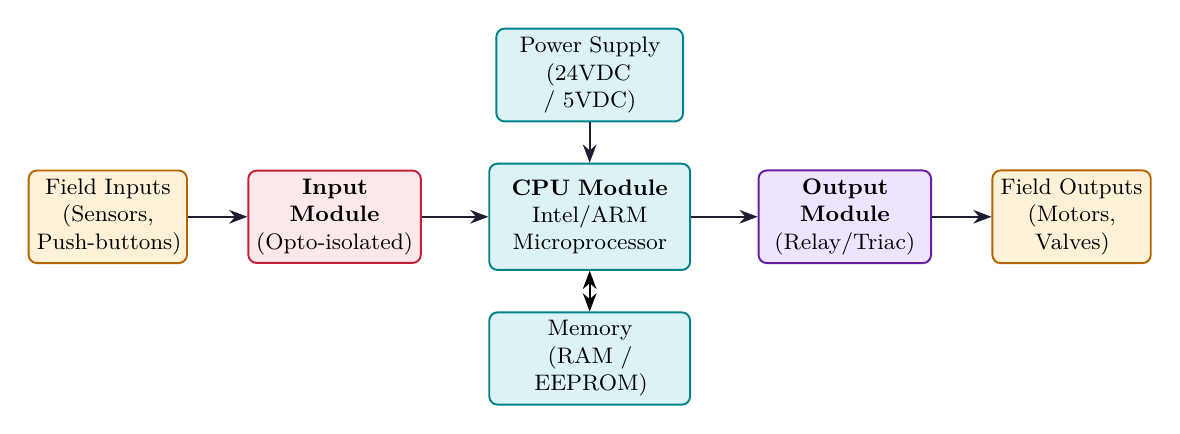
\begin{tikzpicture}[scale=0.9, transform shape]
  % Processor and Memory
  \node[block, text width=2.6cm, minimum height=1.5cm] (cpu) at (0,0) {\textbf{CPU Module}\\Intel/ARM\\Microprocessor};
  \node[block, text width=2.6cm] (mem) at (0, -2.0) {Memory\\(RAM / EEPROM)};
  
  % Input and Output Blocks
  \node[block, draw=myred, fill=hdrred, text width=2.2cm, minimum height=1.3cm] (in) at (-3.6, 0) {\textbf{Input Module}\\(Opto-isolated)};
  \node[block, draw=mypurple, fill=hdrpurple, text width=2.2cm, minimum height=1.3cm] (out) at (3.6, 0) {\textbf{Output Module}\\(Relay/Triac)};
  
  % Field Devices
  \node[block, text width=2.0cm, draw=myamber, fill=hdramber] (dev_in) at (-6.8, 0) {Field Inputs\\(Sensors, Push-buttons)};
  \node[block, text width=2.0cm, draw=myamber, fill=hdramber] (dev_out) at (6.8, 0) {Field Outputs\\(Motors, Valves)};

  % Power Supply
  \node[block, text width=2.4cm] (ps) at (0, 2.0) {Power Supply\\(24VDC / 5VDC)};

  % Internal bus paths
  \draw[Stealth-Stealth, thick] (cpu) -- (mem);
  \draw[arrow] (ps) -- (cpu);
  
  % Input/Output connections
  \draw[arrow] (dev_in) -- (in);
  \draw[arrow] (in) -- (cpu);
  \draw[arrow] (cpu) -- (out);
  \draw[arrow] (out) -- (dev_out);
\end{tikzpicture}
\end{tcolorbox}

\textbf{Core Hardware Blocks:}
\begin{enumerate}[label=\textbf{\arabic*.}, leftmargin=*]
  \item \textbf{CPU Module:} Executes the user program, updates the output image table, and diagnoses system faults.
  \item \textbf{Input Module:} Receives high-voltage field signals (e.g. $120\,$VAC, $24\,$VDC) from pushbuttons or limit switches. It uses \textbf{optical isolation} to convert the signals to low-voltage $5\,$VDC signals, protecting the CPU from electrical noise and voltage spikes.
  \item \textbf{Output Module:} Translates the CPU's logic decisions into power switching to steer load devices (solenoids, contactors, pilot lights).
    \begin{itemize}[leftmargin=*, itemsep=2pt]
      \item \textit{Relay Outputs:} Dry contacts, slow, but switch both AC/DC and handle high currents.
      \item \textit{Transistor outputs (DC only):} Fast solid-state switching, low current.
      \item \textit{Triac outputs (AC only):} Silent solid-state switching, moderate current.
    \end{itemize}
\end{enumerate}

% ===============================================================================
\section{PLC Operational Scan Cycle}
% ===============================================================================

A PLC operates by repeatedly executing a cycle of four distinct phases:

\begin{tcolorbox}[tikzbox, title={PLC Cycle Scan Flow}]
\centering
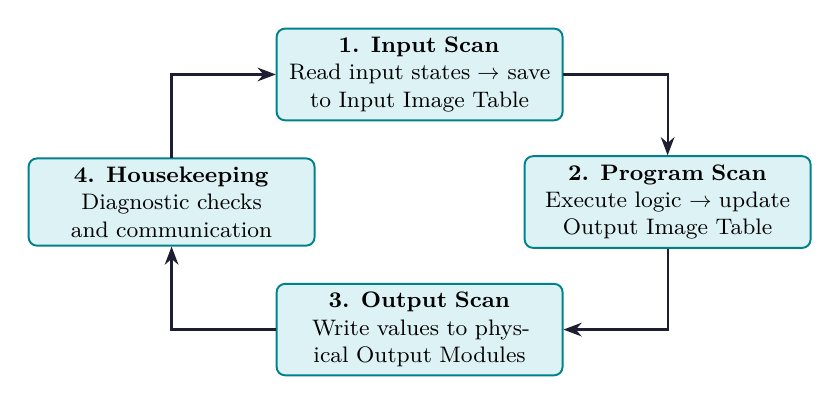
\begin{tikzpicture}[scale=0.9, transform shape]
  % Steps
  \node[block, text width=3.8cm] (step1) at (0, 1.8) {\textbf{1. Input Scan}\\Read input states $\to$ save to Input Image Table};
  \node[block, text width=3.8cm] (step2) at (3.5, 0) {\textbf{2. Program Scan}\\Execute logic $\to$ update Output Image Table};
  \node[block, text width=3.8cm] (step3) at (0, -1.8) {\textbf{3. Output Scan}\\Write values to physical Output Modules};
  \node[block, text width=3.8cm] (step4) at (-3.5, 0) {\textbf{4. Housekeeping}\\Diagnostic checks and communication};

  % Paths
  \draw[arrow] (step1) -| (step2);
  \draw[arrow] (step2) |- (step3);
  \draw[arrow] (step3) -| (step4);
  \draw[arrow] (step4) |- (step1);
\end{tikzpicture}
\end{tcolorbox}

\begin{itemize}[leftmargin=*, itemsep=2.5pt]
  \item \textbf{Scan Time:} The total time required to complete one cycle (typically $1\text{--}10\,$ms).
  \item \textbf{Watchdog Timer:} A hardware timer initialized at the start of each scan cycle. If the scan time exceeds a preset safety limit (e.g. $100\,$ms due to an infinite program loop or processor hang), the watchdog timer trips, instantly shutting down all PLC outputs for safety.
\end{itemize}


% ===============================================================================
\section{Ladder Diagram (LD) Programming}
% ===============================================================================

\subsection{1. Fundamental Instructions}
\begin{itemize}[leftmargin=*, itemsep=2.5pt]
  \item \textbf{Normally Open Contact (NO) \texttt{-[ ]-}:} Examines if a bit is ON (1). If the referenced memory bit is 1, the contact closes, allowing power flow. (Instruction: \textbf{XIC} --- Examine If Closed).
  \item \textbf{Normally Closed Contact (NC) \texttt{-[\textbackslash]-}:} Examines if a bit is OFF (0). If the referenced memory bit is 0, the contact remains closed, allowing power flow. (Instruction: \textbf{XIO} --- Examine If Open).
  \item \textbf{Output Coil \texttt{-( )}-:} Sets a referenced memory bit to 1 when power flows through the rung. (Instruction: \textbf{OTE} --- Output Energize).
  \item \textbf{Latching/Sealing:} Since industrial pushbuttons are momentary, control rungs use a parallel contact of the output coil wired around the start button to "seal in" power.
\end{itemize}

\begin{tcolorbox}[tikzbox, title={Stop-Start Motor Latching Logic (Ladder Diagram)}]
\centering
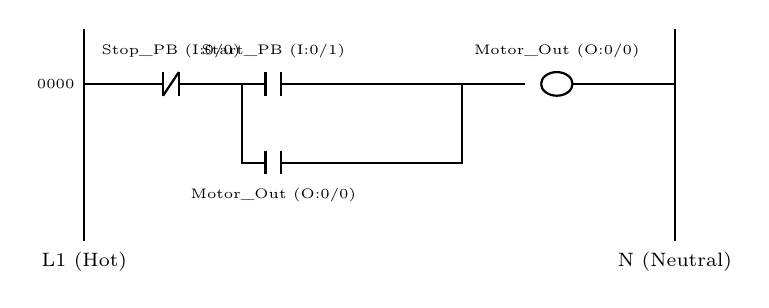
\begin{tikzpicture}[scale=1.0]
  % Rails
  \draw[thick] (0, 1.2) -- (0, -1.5) node[below, font=\scriptsize] {L1 (Hot)};
  \draw[thick] (7.5, 1.2) -- (7.5, -1.5) node[below, font=\scriptsize] {N (Neutral)};
  
  % Rung 1
  \draw[thick] (0, 0.5) -- (0.8, 0.5);
  
  % Stop Contact (NC)
  \draw[thick] (0.8, 0.5) -- (1.0, 0.5);
  \draw[thick] (1.0, 0.35) -- (1.0, 0.65);
  \draw[thick] (1.0, 0.35) -- (1.2, 0.65);
  \draw[thick] (1.2, 0.35) -- (1.2, 0.65);
  \draw[thick] (1.2, 0.5) -- (2.0, 0.5);
  \node[above, font=\tiny] at (1.1, 0.7) {Stop\_PB (I:0/0)};

  % Start Contact (NO)
  \draw[thick] (2.0, 0.5) -- (2.3, 0.5);
  \draw[thick] (2.3, 0.35) -- (2.3, 0.65);
  \draw[thick] (2.5, 0.35) -- (2.5, 0.65);
  \draw[thick] (2.5, 0.5) -- (4.8, 0.5);
  \node[above, font=\tiny] at (2.4, 0.7) {Start\_PB (I:0/1)};
  
  % Seal-in Contact (NO) in parallel
  \draw[thick] (2.0, 0.5) -- (2.0, -0.5) -- (2.3, -0.5);
  \draw[thick] (2.3, -0.65) -- (2.3, -0.35);
  \draw[thick] (2.5, -0.65) -- (2.5, -0.35);
  \draw[thick] (2.5, -0.5) -- (4.8, -0.5) -- (4.8, 0.5);
  \node[below, font=\tiny] at (2.4, -0.7) {Motor\_Out (O:0/0)};
  
  % Output Coil
  \draw[thick] (4.8, 0.5) -- (5.6, 0.5);
  \draw[thick] (5.8, 0.5) arc (0:180:-0.2 and 0.15);
  \draw[thick] (5.8, 0.5) arc (0:180:-0.2 and -0.15);
  \draw[thick] (6.2, 0.5) -- (7.5, 0.5);
  \node[above, font=\tiny] at (6.0, 0.7) {Motor\_Out (O:0/0)};
  
  % Bounding box rung labels
  \node[left, font=\tiny] at (0, 0.5) {0000};
\end{tikzpicture}
\end{tcolorbox}

\subsection{2. Timers and Counters}
\begin{itemize}[leftmargin=*, itemsep=2.5pt]
  \item \textbf{Timer On-Delay (TON):} When the rung becomes true, the timer begins accumulating time. Once the Accumulated Value (ACC) equals the Preset Value (PRE), the \textbf{Done Bit (DN)} is set to 1. If the rung goes false, ACC resets to 0.
  \item \textbf{Timer Off-Delay (TOF):} The DN bit is set to 1 immediately when the rung becomes true. When the rung goes false, the timer starts counting. Once ACC equals PRE, the DN bit resets to 0.
  \item \textbf{Retentive Timer (RTO):} Retains its ACC value even if the rung goes false. A separate \textbf{Reset (RES)} instruction is required to clear ACC back to 0.
  \item \textbf{Counters (CTU/CTD):} Count up (CTU) or down (CTD) on each false-to-true rung transition of their input. The DN bit is set to 1 when ACC matches PRE.
\end{itemize}

% ===============================================================================
\section{Industrial PLC Application Examples}
% ===============================================================================

\subsection{Automatic Tank/Bottle Filling Logic}
\begin{itemize}[leftmargin=*, itemsep=2.5pt]
  \item \textbf{Process Description:} A bottle arrives on a conveyor belt. When the proximity sensor detects the bottle, the conveyor stops, and a solenoid valve opens to fill the bottle. A level sensor detects when the bottle is full, closing the valve and restarting the conveyor.
  \item \textbf{Ladder Logic Allocation:}
    \begin{itemize}[leftmargin=*, itemsep=2pt]
      \item Inputs: \texttt{Start\_PB} (I:0/0), \texttt{Stop\_PB} (I:0/1), \texttt{Prox\_Sensor} (I:0/2), \texttt{Level\_Sensor} (I:0/3).
      \item Outputs: \texttt{Conveyor\_Motor} (O:0/0), \texttt{Fill\_Valve} (O:0/1).
    \end{itemize}
  \item \textbf{Rungs Description:}
    \begin{itemize}[leftmargin=*, itemsep=2pt]
      \item \textbf{Rung 1 (Conveyor Run):} Run the conveyor motor if the system is started, and stop it if the \texttt{Prox\_Sensor} detects a bottle OR the \texttt{Stop\_PB} is pressed.
      \item \textbf{Rung 2 (Fill Valve Run):} Open the fill valve if a bottle is present (\texttt{Prox\_Sensor} is true) and the bottle is not yet full (\texttt{Level\_Sensor} is false).
    \end{itemize}
\end{itemize}

\newpage

% ===============================================================================
% QUICK REVISION PAGE
% ===============================================================================
\begin{center}
  {\large\bfseries\color{myred} Quick Revision --- Module 4}\\[3pt]
  {\small\color{mydark} PLC Systems $|$ PE-EC802B}
\end{center}
\noindent{\color{myred}\rule{\linewidth}{1.2pt}}
\vspace{4pt}

\begin{tcolorbox}[defbox, title={\textbf{One-Line Definitions}}]
\begin{itemize}[leftmargin=*, itemsep=2pt, topsep=0pt]
  \item \textbf{PLC:} A solid-state industrial control computer designed to execute logic programs recursively in real-time.
  \item \textbf{Scan Cycle:} The recursive loop of reading physical inputs, executing code, and updating physical outputs.
  \item \textbf{Watchdog Timer (WDT):} A hardware safety timer that shuts down the PLC if the scan time exceeds a set limit.
  \item \textbf{Optical Isolation:} Using LED-phototransistor pairs to separate high-voltage field wiring from CPU logic circuit.
  \item \textbf{XIC (Examine If Closed):} Contact instruction that is logically true when the referenced memory bit is 1.
  \item \textbf{XIO (Examine If Open):} Contact instruction that is logically true when the referenced memory bit is 0.
  \item \textbf{Seal-in Contact:} A parallel contact of an output coil used to maintain power flow after a momentary button is released.
\end{itemize}
\tcbset{breakable}
\end{tcolorbox}

\begin{tcolorbox}[tikzbox, title={\textbf{Output Module \& Timer Comparisons}}]
\centering
\par\noindent
\renewcommand{\arraystretch}{1.3}
\begin{tabularx}{\linewidth}{|B{3.0cm}|Y|Y|Y|}
\hline
\textbf{Property} & \textbf{Relay Output} & \textbf{Transistor Output} & \textbf{Triac Output} \\ \hline
\textbf{Load Type} & Both AC and DC & DC only & AC only \\ \hline
\textbf{Switch Speed} & Slow ($\sim 10\,$ms) & Very Fast ($< 1\,\mu$s) & Fast (crosses zero, $\sim 8\,$ms) \\ \hline
\textbf{Wear / Lifetime} & Limited (mechanical wear) & Infinite (solid-state) & Infinite (solid-state) \\ \hline
\textbf{Isolation} & Inherently isolated & Requires optocoupler & Requires optocoupler \\ \hline
\end{tabularx}

\vspace{0.3cm}
\begin{tabularx}{\linewidth}{|B{3.0cm}|Y|Y|}
\hline
\textbf{Property} & \textbf{Timer On-Delay (TON)} & \textbf{Timer Off-Delay (TOF)} \\ \hline
\textbf{Enable condition} & Rung must be TRUE to count time & Rung must transition TRUE $\to$ FALSE to count \\ \hline
\textbf{DN Bit Action} & Set to 1 once Preset time is reached & Set to 1 instantly; resets once Preset time is reached \\ \hline
\textbf{Loss of Rung} & ACC value resets instantly to 0 & ACC value resets instantly to 0 \\ \hline
\end{tabularx}
\end{tcolorbox}

\begin{tcolorbox}[exambox, title={\textbf{Frequently Asked / Viva Questions}}]
\begin{enumerate}[leftmargin=*, itemsep=4pt]
  \item \Q{Describe the sequence of operations in a single PLC scan cycle.}
    A scan cycle consists of four sequential steps: (1) \textbf{Input Scan:} reads physical input module terminals and copies states into the Input Image Table. (2) \textbf{Program Scan:} runs the user ladder logic code sequentially, updating the Output Image Table. (3) \textbf{Output Scan:} copies Output Image Table states to the physical output module terminals. (4) \textbf{Housekeeping:} runs communication and processor diagnostics.
  \item \Q{Why is optical isolation used in PLC input modules?}
    Field input devices (limit switches, sensors) operate on high voltages ($24\,$VDC, $120\,$VAC) and are exposed to industrial surges and electromagnetic noise. Optical isolation separates the field wiring from the $5\,$VDC CPU logic using LED-photodiode pairs, preventing high-voltage transients from destroying the processor.
  \item \Q{Compare Relay, Transistor, and Triac output modules in PLCs.}
    Relay output modules are mechanical switches that handle high currents and switch both AC and DC, but are slow and wear out. Transistor output modules are solid-state switches that only handle DC, switch extremely fast, and have an infinite life. Triac output modules are solid-state switches designed for AC only.
  \item \Q{What is the function of the Watchdog Timer (WDT) in a PLC?}
    The WDT is a safety timer that monitors the scan cycle. If the program gets stuck in an infinite loop or the CPU freezes, the scan cycle fails to complete. When the WDT exceeds its preset threshold, it trips, putting the PLC in a "fault" state and turning off all outputs to prevent runaway machine actions.
  \item \Q{State the difference between TON, TOF, and RTO timers.}
    TON (Timer On-Delay) starts counting when its rung becomes true and sets its DN bit when ACC reaches PRE. TOF (Timer Off-Delay) turns on its DN bit immediately when the rung goes true, starts counting when the rung goes false, and resets DN when ACC reaches PRE. RTO (Retentive Timer) behaves like TON but does not reset its ACC value when the rung goes false; it requires an explicit RES instruction.
  \item \Q{How is a seal-in circuit implemented in Ladder Logic, and why is it necessary?}
    It is implemented by wiring a normally open contact of the output coil in parallel with the momentary Start pushbutton contact. When the Start button is pressed, the coil energizes and closes the parallel contact. When the Start button is released, current continues to flow through the parallel contact (sealing it in) until a series Stop pushbutton opens the rung.
\end{enumerate}
\end{tcolorbox}


% -- Module 5 -----------------------------------------------------------------
\modulestart{5}{Distributed Control Systems (DCS) \& SCADA}

\section{Distributed Control Systems (DCS) \& SCADA}
% ===============================================================================

\subsection{1. Distributed Control Systems (DCS)}
A \textbf{DCS} is a control system for a manufacturing plant or process wherein controller functions are distributed throughout the system rather than centralized in a single controller. This distribution provides high scalability, reliability, and ease of loop tuning.

\textbf{1. Hierarchical Architecture (ISA-95 Levels):}
\begin{itemize}[leftmargin=*, itemsep=2.5pt]
  \item \textbf{Level 0 (Field Level):} Sensors (temperature, pressure), actuators, and control valves that interface directly with the process.
  \item \textbf{Level 1 (Direct Control Level):} Distributed controllers (microprocessor-based) that execute fast local PID algorithms and output direct control signals.
  \item \textbf{Level 2 (Supervisory Control Level):} Operators HMIs, supervisory computers, and engineering workstations that manage setpoints, monitor trends, and record alarm logs.
  \item \textbf{Level 3 (Manufacturing Operations Level):} Manufacturing Execution Systems (MES) for production scheduling, quality tracking, and inventory management.
  \item \textbf{Level 4 (Business Planning Level):} Enterprise Resource Planning (ERP) servers for corporate and financial planning.
\end{itemize}

\textbf{2. Functional Requirements:}
A DCS must support the following core functions:
\begin{itemize}[leftmargin=*, itemsep=2pt]
  \item \textbf{Data Acquisition:} Scanning analog and digital inputs from field devices.
  \item \textbf{Continuous Loop Control:} Executing PID loops with cycle times down to $10\,$ms.
  \item \textbf{Alarm Management:} Identifying and sorting process deviations (Hi/Hi-Hi alarms).
  \item \textbf{Historical Archiving:} Long-term logging of variables for audit and safety.
\end{itemize}

\textbf{3. DCS Advantages:}
\begin{itemize}[leftmargin=*, itemsep=2pt]
  \item \textbf{System Reliability (No Single Point of Failure):} Control tasks are isolated. If one controller fails, only its local loops are affected, while the rest of the plant continues running.
  \item \textbf{Redundancy:} High-availability hardware, including redundant processors in hot-standby mode (bumpless transfer under $< 50\,$ms), redundant power grids, and dual-ring communication networks.
  \item \textbf{Modularity and Scalability:} Easier to expand by adding new I/O cards or controllers.
\end{itemize}

\textbf{4. Communication for Distributed Control:}
DCS controllers communicate via deterministic, high-speed industrial networks to guarantee loop synchronization:
\begin{itemize}[leftmargin=*, itemsep=2pt]
  \item \textbf{Fieldbus/Profibus:} For connecting Level 0 field instruments to Level 1 controllers.
  \item \textbf{Industrial Ethernet:} For high-bandwidth communication between Level 1 controllers and Level 2 supervisory HMIs, often configured in a redundant physical ring topology.
\end{itemize}

\textbf{5. DCS Application Examples:}
DCS is ideal for complex, continuous, multi-loop processes:
\begin{itemize}[leftmargin=*, itemsep=2pt]
  \item \textbf{Chemical and Petrochemical Plants:} Monitoring and controlling thousands of interacting pressure, flow, and temperature loops in distillation columns and reactors.
  \item \textbf{Power Generation Plants:} Boiler combustion control, steam turbine regulation, and cooling water loop orchestration.
\end{itemize}

\subsection{2. SCADA Systems}
\textbf{SCADA} (Supervisory Control and Data Acquisition) systems are used to monitor and control large-scale, geographically distributed utility networks (electrical grids, oil/gas pipelines, water networks). Unlike a DCS, SCADA focuses on data collection and supervisory-level control over long distances, leaving local loop execution to local controllers.

\begin{tcolorbox}[tikzbox, title={Geographically Distributed SCADA System Architecture}]
\centering
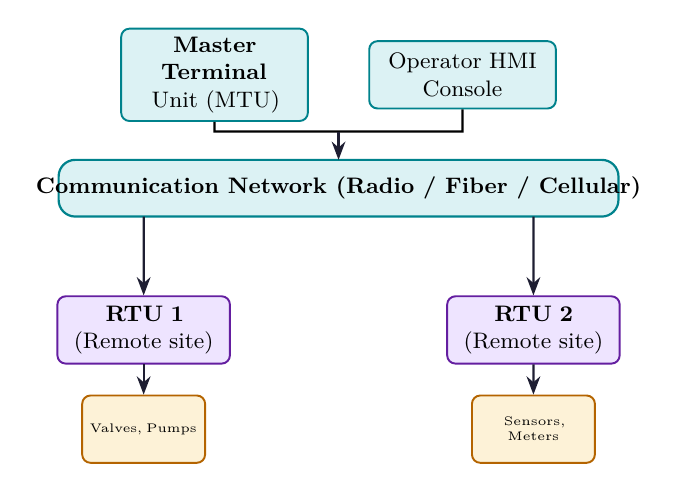
\begin{tikzpicture}[scale=0.9, transform shape]
  % MTU
  \node[block, text width=2.4cm, minimum height=1.2cm] (mtu) at (0, 1.8) {\textbf{Master Terminal}\\Unit (MTU)};
  \node[block, text width=2.4cm] (hmi) at (3.5, 1.8) {Operator HMI\\Console};

  % Communication Cloud
  \draw[thick, draw=myteal, fill=hdrteal, rounded corners=6pt] (-2.2, -0.2) rectangle (5.7, 0.6);
  \node[font=\small\bfseries] at (1.75, 0.2) {Communication Network (Radio / Fiber / Cellular)};

  % RTU 1
  \node[block, text width=2.2cm, draw=mypurple, fill=hdrpurple] (rtu1) at (-1.0, -1.8) {\textbf{RTU 1}\\(Remote site)};
  % RTU 2
  \node[block, text width=2.2cm, draw=mypurple, fill=hdrpurple] (rtu2) at (4.5, -1.8) {\textbf{RTU 2}\\(Remote site)};

  % Field devices
  \node[block, text width=1.5cm, draw=myamber, fill=hdramber, font=\tiny] (dev1) at (-1.0, -3.2) {Valves, Pumps};
  \node[block, text width=1.5cm, draw=myamber, fill=hdramber, font=\tiny] (dev2) at (4.5, -3.2) {Sensors, Meters};

  % Connections
  \draw[thick] (mtu.south) -- (0, 1.0) -- (3.5, 1.0) -- (hmi.south);
  \draw[arrow] (1.75, 1.0) -- (1.75, 0.6);
  
  \draw[arrow] (-1.0, -0.2) -- (rtu1.north);
  \draw[arrow] (4.5, -0.2) -- (rtu2.north);
  
  \draw[arrow] (rtu1) -- (dev1);
  \draw[arrow] (rtu2) -- (dev2);
\end{tikzpicture}
\end{tcolorbox}

\textbf{1. Core Components \& Architecture:}
\begin{itemize}[leftmargin=*, itemsep=2.5pt]
  \item \textbf{MTU (Master Terminal Unit):} The central host server located at the control center. It polls remote stations, archives telemetry data, updates the HMI database, and transmits supervisory commands.
  \item \textbf{RTU (Remote Terminal Unit):} Microprocessor units deployed at remote field sites. They interface with local sensors and actuators, convert signals to digital data, and communicate with the MTU.
  \item \textbf{HMI (Human Machine Interface):} Visual display stations in the control room showing real-time trends, piping \& instrumentation diagrams (P\&ID), and active system alarms.
\end{itemize}

\textbf{2. SCADA Communication \& Telemetry:}
Because SCADA nodes are miles apart, communication is often non-deterministic, using varied media:
\begin{itemize}[leftmargin=*, itemsep=2.5pt]
  \item \textbf{Media:} Radio telemetry, cellular networks (LTE/5G), satellite links, and fiber optics.
  \item \textbf{Polling vs. Event-Driven (Report-by-Exception):} To conserve network bandwidth, SCADA RTUs do not transmit data continuously. In \textbf{Report-by-Exception (RBE)}, the RTU only transmits data if the measured variable changes beyond a preset deadband or if an alarm is triggered.
  \item \textbf{Protocols:} Modbus (legacy, serial/TCP), DNP3 (Distributed Network Protocol, optimized for utilities with time-stamping), and OPC UA (Open Platform Communications Unified Architecture, secure, platform-independent).
\end{itemize}

\textbf{3. SCADA Application Examples:}
SCADA is suited for geographically dispersed networks with low control-loop speeds:
\begin{itemize}[leftmargin=*, itemsep=2pt]
  \item \textbf{Electrical Power Transmission Grids:} Monitoring sub-station switchgears, busbar voltages, and power flow over thousands of square miles.
  \item \textbf{Oil and Gas Pipelines:} Tracking pressure profiles, flow rates, and leak detection across transcontinental pipeline routes, automatically closing remote valves during pressure drops.
  \item \textbf{Water Distribution Systems:} Monitoring water reservoir levels, pipe pressures, and controlling pumping stations across municipal regions.
\end{itemize}


% ===============================================================================
\section{Advanced Industrial Control Techniques}
% ===============================================================================

\subsection{1. Cascade Control}
Cascade control utilizes two nested feedback loops (an inner fast loop and an outer slow loop) to improve disturbance rejection.

\begin{tcolorbox}[tikzbox, title={Cascade Control System Block Diagram}]
\centering
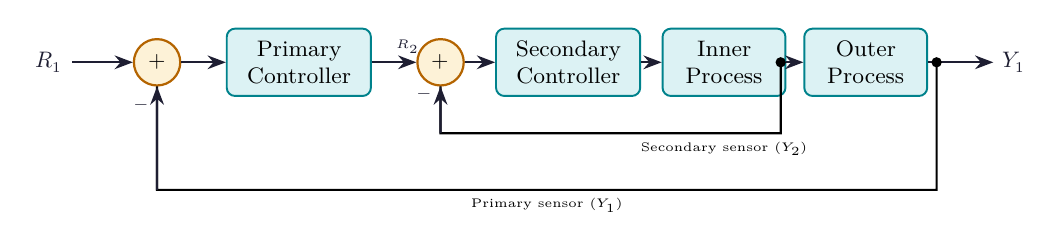
\begin{tikzpicture}[scale=0.9, transform shape]
  % Summer 1 (Outer)
  \node[sumjunc] (sum1) at (-2.0, 0) {$+$};
  \node[block, text width=1.8cm] (ctrl1) at (0, 0) {Primary\\Controller};
  
  % Summer 2 (Inner)
  \node[sumjunc] (sum2) at (2.0, 0) {$+$};
  \node[block, text width=1.8cm] (ctrl2) at (3.8, 0) {Secondary\\Controller};
  
  \node[block, text width=1.5cm] (p1) at (6.0, 0) {Inner\\Process};
  \node[block, text width=1.5cm] (p2) at (8.0, 0) {Outer\\Process};

  % Paths
  \draw[arrow] (-3.2,0) node[left, font=\small] {$R_1$} -- (sum1);
  \draw[arrow] (sum1) -- (ctrl1);
  \draw[arrow] (ctrl1) -- (sum2) node[above, pos=0.8, font=\tiny] {$R_2$};
  \draw[arrow] (sum2) -- (ctrl2);
  \draw[arrow] (ctrl2) -- (p1);
  \draw[arrow] (p1) -- (p2);
  \draw[arrow] (p2) -- (9.8, 0) node[right, font=\small] {$Y_1$};

  % Inner feedback
  \draw[thick] (6.8, 0) to[short, *-] (6.8, -1.0) -| (sum2);
  \draw[arrow] (2.0, -1.0) -- (sum2) node[left, pos=0.8, font=\scriptsize] {$-$};
  \node[below, font=\tiny] at (6.0, -1.0) {Secondary sensor ($Y_2$)};

  % Outer feedback
  \draw[thick] (9.0, 0) to[short, *-] (9.0, -1.8) -| (sum1);
  \draw[arrow] (-2.0, -1.8) -- (sum1) node[left, pos=0.8, font=\scriptsize] {$-$};
  \node[below, font=\tiny] at (3.5, -1.8) {Primary sensor ($Y_1$)};
\end{tikzpicture}
\end{tcolorbox}

\begin{itemize}[leftmargin=*, itemsep=2.5pt]
  \item \textbf{Working:} The outer primary controller computes the setpoint $R_2$ for the inner secondary loop. 
  \item \textbf{Advantage:} Disturbances originating inside the inner loop (e.g. pressure fluctuations in a fuel valve feed) are corrected instantly by the secondary controller before they can affect the primary process output $Y_1$.
\end{itemize}

\subsection{2. Feedforward Control}
Feedforward control measures disturbances ($D$) directly and compensates for them *before* they can affect the process variable ($Y$).

\begin{tcolorbox}[tikzbox, title={Combined Feedforward-Feedback Control System}]
\centering
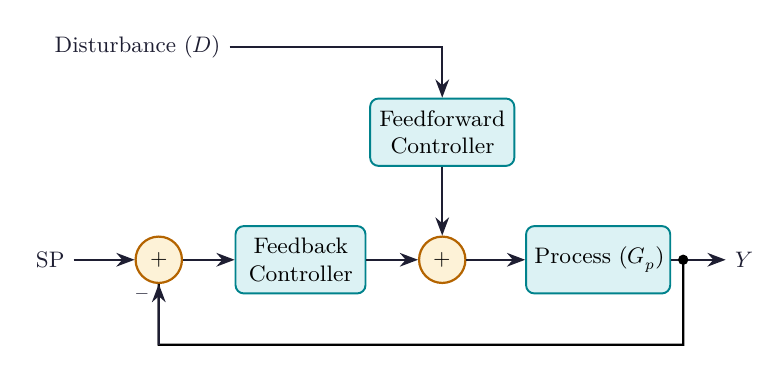
\begin{tikzpicture}[scale=0.9, transform shape]
  \node[sumjunc] (sum1) at (-2.0, 0) {$+$};
  \node[block, text width=1.6cm] (fb) at (0, 0) {Feedback\\Controller};
  \node[sumjunc] (sum2) at (2.0, 0) {$+$};
  \node[block, text width=1.8cm] (proc) at (4.2, 0) {Process ($G_p$)};
  
  \node[block, text width=1.8cm] (ff) at (2.0, 1.8) {Feedforward\\Controller};

  % Paths
  \draw[arrow] (-3.2,0) node[left, font=\small] {SP} -- (sum1);
  \draw[arrow] (sum1) -- (fb);
  \draw[arrow] (fb) -- (sum2);
  \draw[arrow] (sum2) -- (proc);
  \draw[arrow] (proc) -- (6.0, 0) node[right, font=\small] {$Y$};

  % Disturbance feedforward path
  \draw[arrow] (-1.0, 3.0) node[left, font=\small] {Disturbance ($D$)} -- (ff.west |- -1.0, 3.0) -| (ff);
  \draw[arrow] (ff) -- (sum2);
  
  % Feedback loop
  \draw[thick] (5.4, 0) to[short, *-] (5.4, -1.2) -| (sum1);
  \draw[arrow] (-2.0, -1.2) -- (sum1) node[left, pos=0.8, font=\scriptsize] {$-$};
\end{tikzpicture}
\end{tcolorbox}

\begin{itemize}[leftmargin=*, itemsep=2.5pt]
  \item \textbf{Design Equation:} To achieve perfect disturbance cancellation:
    \[
    G_{ff}(s) \cdot G_p(s) + G_d(s) = 0 \Rightarrow G_{ff}(s) = -\frac{G_d(s)}{G_p(s)}
    \]
    where $G_d(s)$ is the disturbance path transfer function and $G_p(s)$ is the process path transfer function.
  \item \textbf{Limitation:} Requires an accurate process model and cannot correct for unmeasured disturbances (hence it is always paired with a feedback controller).
\end{itemize}

\subsection{3. Ratio Control}
Ratio control maintains a fixed ratio between two flows (usually a wild flow $F_w$ and a controlled flow $F_c$, such as fuel-to-air ratio).
\begin{itemize}[leftmargin=*, itemsep=2.5pt]
  \item \textbf{Parallel Configuration:} An operator sets the target total rate; a controller calculates setpoints for both fuel and air flow loops.
  \item \textbf{Series Configuration:} The uncontrolled wild flow is measured, multiplied by a ratio factor $R$, and the result is fed as the setpoint to the controlled flow controller: $SP_c = R \times F_w$.
\end{itemize}

\subsection{4. Split-Range and Override Control}
\begin{itemize}[leftmargin=*, itemsep=2.5pt]
  \item \textbf{Split-Range Control:} A single controller output drives two separate control valves. For example, a $0\text{--}50\%$ output opens a heating steam valve, while $50\text{--}100\%$ opens a cooling water valve.
  \item \textbf{Override (Selective) Control:} Multiple controllers monitor different process variables but output to a single valve. A high/low selector block decides which controller has override authority. Used for limit protection (e.g., maintaining flow rate while overriding to close the valve if pressure exceeds safety limit).
\end{itemize}

\subsection{5. Adaptive Control}
In many industrial processes, the plant dynamics change slowly over time due to wear, temperature drift, aging, or varying operational loads. A standard fixed-parameter PID controller may become unstable or sluggish under these conditions. \textbf{Adaptive control} automatically adjusts the controller parameters online in real-time to maintain desired performance.

\textbf{1. Distinguishing Feature:}
Unlike feedback control (which acts on the error $e(t)$) or feedforward control (which acts on measured disturbances $d(t)$), adaptive control contains a \textbf{parameter adjustment loop} (outer loop) that modifies the controller's gains.

\textbf{2. Core Architectures:}
\begin{itemize}[leftmargin=*, itemsep=2.5pt]
  \item \textbf{Model Reference Adaptive Control (MRAC):}
    \begin{itemize}[leftmargin=*, itemsep=1.5pt]
      \item \textit{Working:} A mathematical \textbf{Reference Model} is chosen to represent the ideal desired closed-loop response. The actual plant output is compared against this reference model output. An adaptation algorithm (e.g., MIT Rule or Lyapunov stability theory) adjusts the controller gains to drive the difference error to zero.
    \end{itemize}
  \item \textbf{Self-Tuning Regulator (STR):}
    \begin{itemize}[leftmargin=*, itemsep=1.5pt]
      \item \textit{Working:} Utilizes a two-step real-time algorithm. First, an online parameter estimator (e.g., Recursive Least Squares --- RLS) identifies the plant's transfer function parameters from input-output data. Second, a controller design block automatically recalculates the controller parameters (e.g., pole placement) based on the newly estimated plant model.
    \end{itemize}
\end{itemize}

\begin{tcolorbox}[tikzbox, title={Model Reference Adaptive Control (MRAC) Architecture}]
\centering
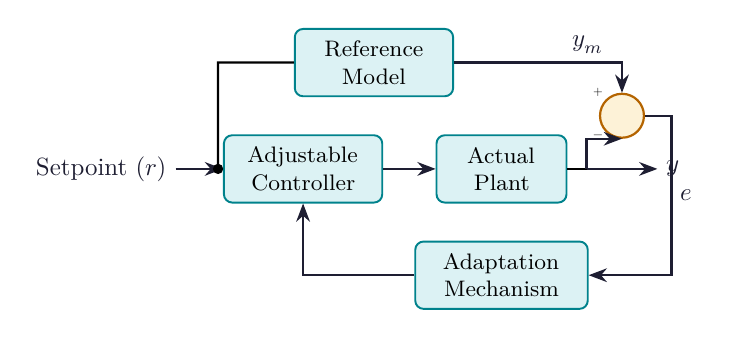
\begin{tikzpicture}[scale=0.9, transform shape]
  % Blocks
  \node[block, text width=2.0cm] (refmodel) at (1.0, 1.5) {Reference\\Model};
  \node[block, text width=2.0cm] (controller) at (0, 0) {Adjustable\\Controller};
  \node[block, text width=1.6cm] (plant) at (2.8, 0) {Actual\\Plant};
  \node[sumjunc] (sum) at (4.5, 0.75) {};
  \node[block, text width=2.2cm] (adapt) at (2.8, -1.5) {Adaptation\\Mechanism};

  % Sign labels on summing junction using anchors to prevent overlaps
  \node[above left, font=\tiny, inner sep=1pt] at (sum.135) {$+$};
  \node[below left, font=\tiny, inner sep=1pt] at (sum.225) {$-$};

  % Paths
  \draw[arrow] (-1.8, 0) node[left] {Setpoint ($r$)} -- (controller);
  \draw[thick] (-1.2, 0) to[short, *-] (-1.2, 1.5) -- (refmodel);
  \draw[arrow] (controller) -- (plant);
  \draw[thick] (plant) -- (4.0, 0);
  \draw[arrow] (4.0, 0) -- (5.0, 0) node[right] {$y$};
  \draw[arrow] (4.0, 0) |- (sum.south);
  \draw[arrow] (refmodel) -| (sum.north) node[above, pos=0.4] {$y_m$};
  \draw[arrow] (sum) -- ++(0.7, 0) |- (adapt) node[right, pos=0.25] {$e$};
  \draw[arrow] (adapt) -| (controller);
\end{tikzpicture}
\end{tcolorbox}

\subsection{6. Internal Model Control (IMC)}
IMC integrates a mathematical model of the process in parallel with the actual plant to predict and reject disturbances.

\begin{tcolorbox}[tikzbox, title={Internal Model Control (IMC) Block Diagram}]
\centering
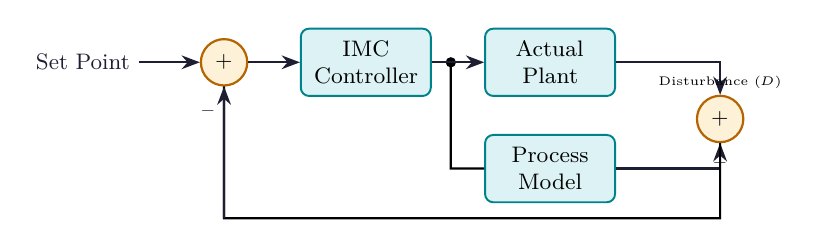
\begin{tikzpicture}[scale=0.9, transform shape]
  \node[sumjunc] (sum1) at (-2.0, 0) {$+$};
  \node[block, text width=1.6cm] (imc) at (0, 0) {IMC\\Controller};
  \node[block, text width=1.6cm] (plant) at (2.6, 0) {Actual\\Plant};
  \node[block, text width=1.6cm] (model) at (2.6, -1.5) {Process\\Model};
  \node[sumjunc] (sum2) at (5.0, -0.8) {$+$};

  % Paths
  \draw[arrow] (-3.2, 0) node[left, font=\small] {Set Point} -- (sum1);
  \draw[arrow] (sum1) -- (imc);
  \draw[thick] (1.2, 0) to[short, *-] (1.2, -1.5) -- (model);
  \draw[arrow] (imc) -- (plant);
  \draw[arrow] (plant) -| (sum2);
  \draw[arrow] (model) -| (sum2) node[below, pos=0.8, font=\scriptsize] {$-$};
  
  \draw[thick] (sum2) -- (5.0, -2.2) -| (sum1);
  \draw[arrow] (-2.0, -2.2) -- (sum1) node[left, pos=0.8, font=\scriptsize] {$-$};
  \node[above, font=\tiny] at (5.0, -0.5) {Disturbance ($D$)};
\end{tikzpicture}
\end{tcolorbox}

\textbf{IMC Controller Design:} If the plant model is $G_m(s)$, the controller is designed as $q(s) = G_m^{-1}(s) \cdot f(s)$, where $f(s)$ is a low-pass filter to guarantee causality and robustness.

\newpage

% ===============================================================================
% QUICK REVISION PAGE
% ===============================================================================
\begin{center}
  {\large\bfseries\color{myred} Quick Revision --- Module 5}\\[3pt]
  {\small\color{mydark} DCS, SCADA \& Advanced Control $|$ PE-EC802B}
\end{center}
\noindent{\color{myred}\rule{\linewidth}{1.2pt}}
\vspace{4pt}

\begin{tcolorbox}[defbox, title={\textbf{One-Line Definitions}}]
\begin{itemize}[leftmargin=*, itemsep=2pt, topsep=0pt]
  \item \textbf{DCS:} A process-oriented control network with distributed processing nodes that handle control loops locally.
  \item \textbf{SCADA:} A geographically wide data acquisition and supervisory system used for utility telemetry and remote control.
  \item \textbf{RTU:} A remote site microprocessor unit that converts field device inputs into telemetry data for SCADA.
  \item \textbf{Feedforward Control:} Open-loop compensation that measures disturbances and takes immediate counter-action.
  \item \textbf{Cascade Control:} A control strategy utilizing nested feedback loops to isolate and reject inner-loop disturbances.
  \item \textbf{Ratio Control:} Control loop configuration maintaining a constant flow ratio between two process streams.
  \item \textbf{Split-Range Control:} Dividing a single controller output range to operate multiple control actuators.
  \item \textbf{Adaptive Control:} A control scheme that automatically adjusts controller parameters in real-time to adapt to changing plant dynamics.
  \item \textbf{Report-by-Exception:} A SCADA communication scheme where remote nodes only transmit data if a value changes beyond a preset limit.
\end{itemize}
\end{tcolorbox}

\begin{tcolorbox}[tikzbox, title={\textbf{Industrial Control Strategy Comparisons}}]
\centering
\par\noindent
\renewcommand{\arraystretch}{1.3}
\begin{tabularx}{\linewidth}{|B{3.0cm}|Y|Y|}
\hline
\textbf{Property} & \textbf{Distributed Control System (DCS)} & \textbf{SCADA System} \\ \hline
\textbf{Syllabus Focus} & Process-oriented (fast loop control, DCS controllers) & Data-oriented (telemetry, remote monitoring) \\ \hline
\textbf{Distribution} & Locally distributed within a plant site & Geographically distributed over wide areas \\ \hline
\textbf{Communication} & Fast, deterministic networks (Ethernet/control rings) & Slow, non-deterministic links (radio, GSM, satellite) \\ \hline
\textbf{Closed-loop Control} & Executes direct loops at controller level & Executes supervisory control (manual/slow setpoint tuning) \\ \hline
\end{tabularx}

\vspace{0.3cm}
\begin{tabularx}{\linewidth}{|B{3.0cm}|Y|Y|}
\hline
\textbf{Property} & \textbf{Feedback Control} & \textbf{Feedforward Control} \\ \hline
\textbf{Control Action} & Corrective (acts *after* output deviates) & Preventive (acts *before* disturbance affects plant) \\ \hline
\textbf{Stability Risk} & High (gain can drive phase delay oscillations) & None (does not introduce feedback poles) \\ \hline
\textbf{Model Requirement} & No model needed (easy PID tuning) & Requires high-accuracy process model ($G_d/G_p$) \\ \hline
\end{tabularx}
\end{tcolorbox}

\begin{tcolorbox}[exambox, title={\textbf{Frequently Asked / Viva Questions}}]
\begin{enumerate}[leftmargin=*, itemsep=4pt]
  \item \Q{Compare DCS and SCADA in terms of architecture and applications.}
    DCS is process-oriented, localized (within a single facility like a chemical plant), and executes fast, closed-loop control over high-bandwidth networks. SCADA is data-oriented, geographically distributed (over thousands of kilometers like a power grid), and relies on low-bandwidth telemetry (radio, GSM) for supervisor-level monitoring and slow-loop adjustments.
  \item \Q{How does Cascade Control improve disturbance rejection?}
    In cascade control, the secondary inner loop operates much faster than the primary outer loop. If a disturbance enters the secondary loop (e.g. feed pressure drops), the secondary controller corrects it immediately before the disturbance can propagate and affect the primary process output.
  \item \Q{Derive the transfer function of an ideal feedforward controller.}
    Let $Y = G_p U + G_d D$ be the process output, where $U$ is control input, $D$ is disturbance, and $G_p, G_d$ are transfer functions. In feedforward control, $U = G_{ff} D$. Substituting $U$ gives $Y = (G_p G_{ff} + G_d) D$. For perfect disturbance cancellation, we require $Y=0$ for any $D \Rightarrow G_p G_{ff} + G_d = 0 \Rightarrow G_{ff}(s) = -G_d(s)/G_p(s)$.
  \item \Q{What is ratio control, and where is it used?}
    Ratio control is an advanced control strategy that maintains a constant ratio between two variable flows (usually fuel and air, or two blending chemicals). It measures a "wild" uncontrolled flow and adjusts a "controlled" flow to match the predefined ratio, preventing incomplete combustion or mixing errors.
  \item \Q{Explain the concept of Split-Range Control with an example.}
    Split-range control splits the output range of a single controller to command multiple actuators. For example, in a reactor temperature loop, a $0\text{--}100\%$ controller output is split: $0\text{--}50\%$ operates a steam valve (for heating), and $50\text{--}100\%$ operates a cooling water valve (for cooling).
  \item \Q{What is Internal Model Control (IMC), and what is its main advantage?}
    IMC is a control structure where a mathematical model of the process is run in parallel with the actual plant. The difference between the plant and model outputs is fed back as an estimate of the net disturbance. This structure simplifies controller design, allows direct control of delays, and guarantees robustness.
  \item \Q{Explain the difference between Model Reference Adaptive Control (MRAC) and Self-Tuning Regulator (STR).}
    MRAC compares the plant's output against the output of a predefined reference model and uses the difference (error) to adjust the controller parameters. STR uses an online parameter estimator (like recursive least squares) to identify the plant parameters in real-time, then recalculates the controller parameters based on the estimated model.
  \item \Q{What is Report-by-Exception (RBE) in SCADA, and why is it used?}
    RBE is an event-driven telemetry scheme where remote terminal units (RTUs) only transmit data to the master terminal unit (MTU) if a variable deviates beyond a preset deadband or if an alarm occurs. It is used to conserve network bandwidth over slow, costly, or congested communication links (like radio or satellite).
\end{enumerate}
\end{tcolorbox}


\end{document}
